\documentclass[11pt]{article}
\usepackage{amsmath,amssymb,amsfonts,amsthm}
\usepackage{graphicx}
\usepackage{cite}
\usepackage{algorithm,algorithmic}
\usepackage{times}
\usepackage{fancyhdr}
\usepackage[small]{titlesec}
\usepackage{color}
\usepackage{enumerate}

\pagestyle{fancy}

\oddsidemargin=0.0in %%this makes the odd side margin go to the default of 1inch
\evensidemargin=0.0in
\textwidth=6.5in
\headwidth=6.5in
\textheight=9in %%sets the textwidth to 6.5, which leaves 1 for the remaining right margin with 8 1/2X11inch paper
\headheight=12pt
\topmargin=-0.25in


\usepackage{hyperref}
\hypersetup{
    linkcolor=red,          % color of internal links
    citecolor=green,        % color of links to bibliography
    filecolor=magenta,      % color of file links
    urlcolor=cyan           % color of external links
}


\newcommand{\jv}{Joshua Vogelstein}
\newcommand{\jhu}{Johns Hopkins University}
%\newcommand{\hp}{https://jshare.johnshopkins.edu/jvogels3/public_html/}
\newcommand{\ema}{joshuav@jhu.edu}

\newcommand{\Vr}{V_{reset}}
\newcommand{\Vl}{V_{leat}}
\newcommand{\eqdef}{\overset{\triangle}{=}}
% \newcommand{\D}[2]{\frac{\partial #1}{\partial #2}}
\newcommand{\dd}[2]{\frac{\partial ^2 #1}{\partial #2 ^2}}
\newcommand{\DDD}[3]{\frac{\partial ^2 #1}{\partial #2 \partial #3}}
\newcommand{\Di}[2]{\frac{\partial ^i #1}{\partial #2 ^i}}
\newcommand{\grad}{\nabla}
\newcommand{\Hess}{\nabla\nabla}
\newcommand{\defn}{\overset{\triangle}{=}}

\providecommand{\tg}[1]{\textcolor{green}{#1}}
\providecommand{\tb}[1]{\textcolor{blue}{#1}}
\providecommand{\tr}[1]{\textcolor{red}{#1}}
\providecommand{\tk}[1]{\textcolor{black}{#1}}
\providecommand{\twhite}[1]{\textcolor{white}{#1}}
\providecommand{\ve}[1]{\boldsymbol{#1}}
\providecommand{\ma}[1]{\boldsymbol{#1}}
%\providecommand{\ve}[1]{\boldsymbol{#1}}
%\newcommand{\norm}[1]{\left|\left|#1\right|\right|}
\providecommand{\norm}[1]{\left \lVert#1 \right  \rVert}
\providecommand{\deter}[1]{\lvert #1 \rvert}
\providecommand{\abs}[1]{\left \lvert #1 \right \rvert}
\providecommand{\mat}[1]{\left[ #1 \right]}
\newcommand{\trans}[1]{{#1}^{\ensuremath{\mathsf{T}}}}           % transpose
\newcommand{\transpose}[1]{{#1}^{\ensuremath{\mathsf{T}}}}           % transpose
\newcommand{\argmax}{\operatornamewithlimits{argmax}}
\newcommand{\argmin}{\operatornamewithlimits{argmin}}
\newcommand{\T}{^{\ensuremath{\mathsf{T}}}}           % transpose
\newcommand{\from}{{\ensuremath{\colon}}}           % :

\newcommand{\Aa}{\mathbb{A}}
\newcommand{\BB}{\mathbb{B}}
\newcommand{\CC}{\mathbb{C}}         
\newcommand{\DD}{\mathbb{D}}         
\newcommand{\EE}{\mathbb{E}}           % expected value
\newcommand{\FF}{\mathbb{F}}         
\newcommand{\GG}{\mathbb{G}}
\newcommand{\HH}{\mathbb{H}}         
\newcommand{\II}{\mathbb{I}}           % indicator function
\newcommand{\LL}{\mathbb{L}}
\newcommand{\MM}{\mathbb{M}}
\newcommand{\NN}{\mathbb{N}}
\newcommand{\PP}{\mathbb{P}}         
\newcommand{\QQ}{\mathbb{Q}}           
\newcommand{\SSS}{\mathbb{S}}           
\newcommand{\VV}{\mathbb{V}}
\newcommand{\XX}{\mathbb{X}}         
\newcommand{\YY}{\mathbb{Y}}
\newcommand{\ZZ}{\mathbb{Z}}         

\newcommand{\iid}{\overset{iid}{\sim}}
\newcommand{\knn}{$k$NN}

% \DeclareMathOperator*{\argmax}{argmax}
% \DeclareMathOperator*{\argmin}{argmin}
% \DeclareMathOperator{\find}{find}

% \newtheorem{thm}{Theorem}
\newcommand{\thma}{\begin{thm}}
\newcommand{\thmb}{\end{thm}}

\newcommand{\mata}{\begin{bmatrix}}
\newcommand{\matb}{\end{bmatrix}}



\newtheorem{Rem}{Remark}%[section]
\newtheorem{Alg}{Algorithm}%[section]
\newtheorem{thm}{Theorem}
\newtheorem{lem}{Lemma}
\newtheorem{Thm}{Theorem}[section]
\newtheorem{Lem}{Lemma}%[section]
\newtheorem{defi}{Definition}
\newtheorem{Def}{Definition}[section]
\newtheorem{prop}{Proposition}
\newtheorem{coro}[thm]{Corollary}
\newtheorem{claim}{Claim}
\newtheorem{conj}{Conjecture}
\newtheorem{question}{Question}

% \newtheorem{corollary}{Corollary}
% \newtheorem{theorem}{Theorem}
%\theoremstyle{marginbreak}
%\newtheorem{Lem}[Cor]{Lemma}
%\theoremstyle{change}
%\theorembodyfont{\itshape}


% \newtheorem{defi}{Definition}
% \newcommand{\defa}{\begin{defi}}
% \newcommand{\defb}{\end{defi}}

% \newcommand{\eq}{\begin{equation}}
% \newcommand{\en}{\end{equation}}
% \newcommand{\eqa}{\begin{equation}}
% \newcommand{\eqb}{\end{equation}}

\newcommand{\enuma}{\begin{enumerate}}
\newcommand{\enumb}{\end{enumerate}}
\newcommand{\ena}{\begin{enumerate}}
\newcommand{\enb}{\end{enumerate}}

\newcommand{\itema}{\begin{itemize}}
\newcommand{\itemb}{\end{itemize}}
\newcommand{\ita}{\begin{itemize}}
\newcommand{\itb}{\end{itemize}}

% \newcommand{\aligna}{\begin{align}}
% \newcommand{\alignb}{\end{align}}

\newcommand{\proofa}{\begin{proof}}
\newcommand{\proofb}{\end{proof}}

\newcommand{\bla}{\begin{block}}
\newcommand{\blb}{\end{block}}

% \newcommand{\seqa}{\begin{equation*}}
\newcommand{\seqb}{\end{equation*}}

\newcommand{\bth}{\ve{\theta}}
\newcommand{\hth}{\mh{\theta}}
\newcommand{\htth}{\mh{\theta}}
\newcommand{\bhth}{\mh{\ve{\theta}}}
\newcommand{\thetn}{\ve{\theta}}
\newcommand{\thet}{\thetn}
\newcommand{\theth}{\widehat{\ve{\theta}}}
\newcommand{\theto}{\ve{\theta}'}
\newcommand{\wht}{\widehat{\thet}}
\newcommand{\wtt}{\widetilde{\thet}}
\newcommand{\vth}{\ve{\thet}}
\newcommand{\vTh}{\ve{\Theta}}
\newcommand{\hvth}{\widehat{\ve{\thet}}}
\newcommand{\bTh}{\ve{\Theta}}
\newcommand{\hbth}{\widehat{\thet}}
\newcommand{\tbth}{\tilde{\bth}}

% \newcommand{\p}{P_{\bth}}
\newcommand{\pold}{P_{\bth'}}
\newcommand{\pk}{P_{\widehat{\ve{\theta}}^{(k)}}}
\newcommand{\pT}{P_{\thetn_{Tr}}} %\thetn_T
\newcommand{\pO}{P_{\thetn_o}} %\thetn_o
% \newcommand{\Q}{Q(\thetn,\theto)}
% \newcommand{\m}{m^{\ast}}
% \newcommand{\q}{q(\ve{H}_t)}
\newcommand{\Ca}{[\text{Ca}^{2+}]}

\newcommand{\Lik}{\mathcal{L}}
\newcommand{\Cae}{[\widehat{\text{Ca}}^{2+}]}
\newcommand{\Cav}{\ve{C}}%[\ve{\text{Ca}}^{2+}]}
\newcommand{\sml}{\sqrt{\ma{\lambda}}}
\newcommand{\ml}{\ma{\lambda}}
\newcommand{\nw}{\widehat{n}}
\newcommand{\nv}{\vec{n}}
\newcommand{\Ae}{\widehat{A}}
\newcommand{\te}{\widehat{\tau}}
\newcommand{\maxn}{\max_{\ve{n}: n_t \geq 0}}
% \newcommand{\V}{\text{Var}}

\providecommand{\ms}[1]{\mathsf{#1}}
\providecommand{\mc}[1]{\mathcal{#1}}
\providecommand{\mb}[1]{\boldsymbol{#1}}
\providecommand{\mbb}[1]{\mathbb{#1}}
\providecommand{\mv}[1]{\vec{#1}}
\providecommand{\mh}[1]{\hat{#1}}
\providecommand{\wh}[1]{\widehat{#1}}
\providecommand{\mhv}[1]{\mh{\mv{#1}}}
\providecommand{\mvh}[1]{\mv{\mh{#1}}}
\providecommand{\mt}[1]{\widetilde{#1}}
\providecommand{\mhc}[1]{\hat{\mathcal{#1}}}
\providecommand{\mbc}[1]{\mb{\mathcal{#1}}}
\providecommand{\mvc}[1]{\mv{\mathcal{#1}}}
\providecommand{\mtc}[1]{\widetilde{\mathcal{#1}}}
\providecommand{\mth}[1]{\mt{\mh{#1}}}
\providecommand{\mht}[1]{\mh{\mt{#1}}}
\providecommand{\mhb}[1]{\hat{\boldsymbol{#1}}}
\providecommand{\whb}[1]{\widehat{\boldsymbol{#1}}}
\providecommand{\mvb}[1]{\vec{\boldsymbol{#1}}}
\providecommand{\mtb}[1]{\widetilde{\boldsymbol{#1}}}

\newcommand{\PmcP}{P \in \mc{P}}
\newcommand{\mP}{\mathbb{P}}

\newcommand{\del}{\delta}
\newcommand{\sig}{\sigma}
\newcommand{\lam}{\lambda}
\newcommand{\gam}{\gamma}
\newcommand{\eps}{\varepsilon}

\newcommand{\Del}{\Delta}
\newcommand{\Sig}{\Sigma}
\newcommand{\Lam}{\Lambda}
\newcommand{\Gam}{\Gamma}

\newcommand{\dvs}{\dot{\bs}_t}
\newcommand{\dvw}{\dot{\bw}_t}
\newcommand{\dvx}{\dot{\bx}_t}
\newcommand{\dvy}{\dot{\by}_t}

\newcommand{\ft}{f_{\ve{\thet}}}
\newcommand{\gt}{g_{\ve{\thet}}}
\newcommand{\hht}{h_{\thetn}}

\newcommand{\Real}{\mathbb{R}}

\newcommand{\wconv}{\overset{i.p.}{\rightarrow}}
\newcommand{\sconv}{\overset{i.p.}{\rightarrow}}
\newcommand{\conv}{\rightarrow}
\newcommand{\pconv}{\overset{p}{\conv}}
\newcommand{\mcE}{\mathcal{E}}
\newcommand{\mcT}{\mathcal{T}}
\newcommand{\mcG}{\mathcal{G}}
\newcommand{\mcM}{\mathcal{M}}
\newcommand{\mcL}{\mathcal{L}}
\newcommand{\hatmcE}{\widehat{\mcE}}
\newcommand{\hatp}{\widehat{p}}
\newcommand{\hatP}{\widehat{P}}
\newcommand{\hatQ}{\widehat{Q}}
\newcommand{\hatL}{\widehat{L}}
\newcommand{\mhP}{\widehat{\PP}}
\newcommand{\tildeA}{\widetilde{A}}

\newcommand{\defa}{\begin{defi}}
\newcommand{\defb}{\end{defi}}
\newcommand{\defeq}{\overset{\triangle}{=}}


% \newcommand{\ss}{\mc{S}}
% \newcommand{\mhc}{\mh{\mc{S}}_n}

% \newcommand{\Real}{\mathbb{R}}
% \newcommand{\bTh}{\mb{\Theta}}
% \newcommand{\ra}{\rightarrow}
% \newcommand{\la}{\leftarrow}
\newcommand{\bX}{\mb{X}}

% \newcommand{\bv}{\mb{v}}
% \newcommand{\ba}{\mb{a}}
% \newcommand{\bd}{\mb{d}}
% \newcommand{\balpha}{\mb{\alpha}}
% \newcommand{\conv}{\rightarrow}  
% \newcommand{\xx}{\langle \bx_u^\la, \bx_v^\ra\rangle}  
% \DeclareMathOperator*{\argmax}{arg \hspace{1pt} max \hspace{2pt}}
% \DeclareMathOperator*{\argmin}{arg \hspace{1pt} min \hspace{2pt}}
% \newcommand{\norm}[1]{\left \lVert#1 \right  \rVert}
% 


\newcommand{\theHalgorithm}{\arabic{algorithm}}


\DeclareMathOperator{\Delti}{\mathbf{\Delta}^{-1}}
\DeclareMathOperator{\Delt}{Q} %\mathbf{\Delta}}
% \DeclareMathOperator{\Gam}{\mathbf{\Gamma}}
\DeclareMathOperator{\Gami}{\mathbf{\Gamma}^{-1}}
\DeclareMathOperator{\Sigb}{\mathbf{\Sigma}}
\DeclareMathOperator{\Ri}{\mathbf{\R}^{-1}}
\DeclareMathOperator{\A}{A}
\DeclareMathOperator{\W}{\mathbf{W}}
\DeclareMathOperator{\V}{\mathbf{V}}
\DeclareMathOperator{\U}{\mathbf{U}}
\DeclareMathOperator{\C}{\mathbf{C}}
\DeclareMathOperator{\uvec}{\mathbf{u}}
\DeclareMathOperator{\D}{\mathbf{D}}
\DeclareMathOperator{\Q}{\mathbf{Q}}
\DeclareMathOperator{\R}{R} %\mathbf{P}}
\DeclareMathOperator{\Y}{\mathbf{Y}}
\DeclareMathOperator{\B}{\mathbf{B}}
\DeclareMathOperator{\Hmat}{\mathbf{H}}
\DeclareMathOperator{\Gmat}{\mathbf{G}}
\DeclareMathOperator{\X}{\mathbf{X}}
\DeclareMathOperator{\Cmat}{C} %\mathbf{L}}
\DeclareMathOperator{\Pmat}{\mathbf{P}}
\DeclareMathOperator{\veta}{\mathbf{\mb{v}}}
\DeclareMathOperator*{\minimize}{\mathrm{minimize}}
\DeclareMathOperator*{\maximize}{\mathrm{maximize}}
\DeclareMathOperator*{\Ymod}{\mathbf{\Y}}
\DeclareMathOperator*{\Bmod}{\mathbf{B}}
\DeclareMathOperator*{\Hmod}{\mathbf{H}}
\DeclareMathOperator*{\Lmod}{\mathbf{L}}
\DeclareMathOperator*{\Xmod}{\mathbf{\X}}
% \DeclareMathOperator*{\mb{v}mod}{\mathbf{\mb{v}}}

\newcommand{\elegans}{\emph{C. elegans} }

\newcommand{\FAQ}{\texttt{FAQ} }

\providecommand{\tg}[1]{\textcolor{green}{#1}}
\providecommand{\tb}[1]{\textcolor{blue}{#1}}
\providecommand{\tr}[1]{\textcolor{red}{#1}}

\newcommand{\Qs}{Q}
\newcommand{\mcS}{\mc{S}}
\newcommand{\mcU}{\mc{U}}

\newcommand{\mbd}{\mb{d}}
\newcommand{\mbD}{\mb{D}}
\newcommand{\mbx}{\mb{x}}
\newcommand{\mbX}{\mb{X}}
\newcommand{\mby}{\mb{y}}
\newcommand{\mbY}{\mb{Y}}

\newcommand{\mtbd}{\mtb{d}}
\newcommand{\mtbD}{\mtb{D}}
\newcommand{\mtbx}{\mtb{x}}
\newcommand{\mtbX}{\mtb{X}}
\newcommand{\mtby}{\mtb{y}}
\newcommand{\mtbY}{\mtb{Y}}

\floatname{algorithm}{Procedure}
\renewcommand{\algorithmicrequire}{\textbf{Input:}}
\renewcommand{\algorithmicensure}{\textbf{Output:}}
\floatname{algorithm}{Pseudocode}
% \usepackage{longtable}

\title{\vspace{-75pt}Large (Brain) Graph Matching via \\ Fast Approximate Quadratic Programming}
\author{Joshua T.~Vogelstein, John M.~Conroy, Louis J.~Podrazik, Steven G.~Kratzer, Eric T.~Harley, \\
        Donniell E.~Fishkind, 
		R.~Jacob~Vogelstein,
        and~Carey~E.~Priebe}

\begin{document}
\maketitle

 
\begin{abstract}
	
Graph matching (GM)---the process of finding an optimal permutation of the vertices of one graph to minimize adjacency disagreements with the vertices of another---is rapidly becoming an increasingly important computational problem, arising in fields ranging from machine vision to neuroscience. Because GM is $\mc{NP}$-hard, exact algorithms are unsuitable for today's large graphs (with $\ge 1000$ vertices). 
Approximate algorithms necessarily employ a accuracy/efficiency trade-off.
We developed a fast approximate quadratic assignment algorithm (\texttt{FAQ}). 
\FAQ scales cubicly with the number of vertices, similar to other approximate GM algorithms.  Our formulation, however, achieves a lower objective function value than all previously proposed algorithms on over $93\%$ of the QAPLIB benchmark problems.  Moreover, our algorithm runs faster than the second best algorithm on over $80\%$ of the benchmarks.  
We therefore implement our algorithm on a dataset of increasing interest to the neurobiology community: the brain-graph (connectome) of the C. elegans. \FAQ solves this problem perfectly, and no other algorithm we tried was successful.  
Future work will hopefully improve upon the cubic complexity of \FAQ to be able to match mammalian brain-graphs, with millions or billions of vertices.  
\end{abstract}




\section{Introduction}

Graph matching---the process of finding an optimal permutation of the vertices of one graph to minimize adjacency disagreements with the vertices of another---is a famously computationally daunting problem (see, for example, ``Thirty Years of Graph Matching in Pattern Recognition''  \cite{Conte2004}). Specifically, graph matching is an $\mc{NP}$-hard problem, in particular, we do not know whether a polynomial time algorithm can solve it in worst case scenarios \cite{Papadimitriou1998}.  
% Perhaps the most prominent special case of graph matching is the traveling salesman problem \cite{Burkard2009}. 
As such, performance of graph matching algorithms are usually evaluated on graphs with $\dot{\approx} 10$ vertices, or at maximum $\dot{\approx} 100$ (see \cite{Burkard1997} for a description of the standard set of benchmarks).  Yet, it is increasingly popular to represent large data sets by a graph, and thus increasingly desirable to consider matching large graphs.  

The motivating application for this work is \emph{brain-graph matching}.  A brain-graph (aka, a connectome) is a graph for which vertices represent (collections of) neurons and edges represent connections between them \cite{SpornsKotter05, Hagmann05}. Via  Magnetic resonance (MR) imaging, one can image the whole brain and estimate connectivity across voxels, yielding a voxelwise connectome with up to $\dot{\approx} 10^6$ vertices and $\dot{\approx} 10^9$ edges \cite{Zuo2011}.  Comparing brains is an important step for many neurobiological inference tasks.  For example, it is becoming increasingly popular to diagnose neurological diseases via comparing brain images \cite{Csernansky2004}.  To date, however, these comparisons have largely rested on anatomical (e.g., shape) comparisons, not graph comparisons.  This is despite the widely held doctrine that many
% Yet almost immediately after the ``neuron doctrine'' was conjectured (the idea that networks of neurons comprise brains), Wernicke and others began postulating that 
psychiatric disorders are fundamentally ``connectopathies'', that is, disorders of the connections of the brain \cite{Kubicki2007,Calhoun2011,Fornito2012,Fornito2012a}. Currently available tests for connectopic explanation of psychiatric disorders  hedge upon first choosing some number of graph invariants to compare across populations. The graph invariant approach to classifying is both theoretically and practically inferior to comparing whole graphs via matching \cite{VP11_unlabeled}.  

More generally, state-of-the-art inference procedures for essentially any decision-theoretic or inference task follow from constructing interpoint dissimilarity matrices, or graphs \cite{Duin2011}.  Thus, we believe that graph matching of large graphs will become a fundamental subroutine of many statistical inference pipelines operating on graphs. Because the number of vertices of these graphs is so large, exact matching is intractable.   Instead, we require inexact matching algorithms (also called ``heuristics'') that will scale polynomially or even linear \cite{Conte2004}.  In developing such algorithms, there is an inherent accuracy/efficiency trade-off.  If an algorithm outperforms another on both dimensions, it is clearly preferential.  

The remainder of this paper is organized as follows.  Section \ref{sec:GM} formally defines the ``graph matching'' problem, and Section \ref{sec:QAP} makes the connection between graph matching and quadratic assignment problems (QAPs).  Section \ref{sec:FAQ} describes our algorithm, a Fast Approximate QAP (\texttt{FAQ}).  Section \ref{sec:results} provides a number of theoretical and empirical results, comparing our algorithm to previous state-of-the-art algorithms in terms of both computational efficiency and objective function value.  We conclude with a discussion in Section \ref{sec:discussion}.
% In the sequel, we describe our fast approximate quadratic assignment algorithm called \texttt{FAQ} and demonstrate its superior performance relative to its predecessors.  
% We develop an approach to graph matching based on a relaxation of the quadratic programming problem (QAP), which is cubic in the number of vertices, and outperforms previously proposed approximate graph matching heuristics on a wide range of benchmark datasets as well as our motivating application.  




\section{Graph Matching} % (fold)
\label{sec:GM}


A labeled graph $G=(\mc{V},\mc{E})$ consists of a vertex set $\mc{V}$, where $|\mc{V}|=n$ is number of vertices, and an edge set $\mc{E}$. %, where $|\mc{E}| \leq n^2$. 
Note that we are not restricting our formulation to be directed or exclude self-loops. Given a pair of graphs, $G_A=(\mc{V}_A,\mc{E}_A)$ and $G_B=(\mc{V}_B,\mc{E}_B)$, where $|\mc{V}_A|=|\mc{V}_B|=n$, 
let $\Pi$ be the set of permutation functions (bijections), $\Pi=\{\pi \from \mc{V}_A \to \mc{V}_B\}$.
% $\pi: \mc{V}_1 \to \mc{V}_2$ be a permutation function (bijection), and let $\Pi$ be the set of all such permutation functions.  
Now consider the following two closely related problems:
% A pair of graphs, $G_1$ and $G_2$, are isomorphic if and only if the following \emph{isomorphism criterion} holds: there exists a $\pi \in \Pi$ such that . 
% Let $A$ be the adjacency matrix representation of graph such that $A_{ij}=1$ if there is an edge from $u$ to $v$, and $A_{ij}=0$ otherwise. 
% Note that the below follows for directed/undirected and loopy/non-loopy graphs.
% $u \sim v \in \mc{E}$ and $A_{ij}=0$ otherwise.  
% Let  $\Pi$ be the set of permutation functions, where a permutation function (bijection) $\pi: \mc{V} \to \mc{V}$ (re-)orders the elements of the set $\mc{V}$.  Given a pair of $n \times n$ adjacency matrices, $A=(a_{ij})$ and $B=(b_{ij})$, consider the following two problems:
\begin{itemize}
	\item \textbf{Graph Isomorphism (GI):}  Does there exist a $\pi \in \Pi$ such that $(u,v) \in \mc{E}_A$ if and only if $(\pi(u),\pi(v)) \in \mc{E}_B$. 
		\item \textbf{Graph Matching (GM):}
		% Which $\pi \in \Pi$ minimizes the number of pairs of vertices $u,v \in \mc{V}_A$ such that $(u,v) \in \mc{E}_A$ and $(\pi (u) ,\pi (v)) \not \in \mc{E}_B$ or $(u,v) \not \in \mc{E}_A$ and  $(\pi (u) ,\pi (v)) \in \mc{E}_B$
		 Which $\pi \in \Pi$ minimizes adjacency disagreements between $\mc{E}_A$ and the permuted $\mc{E}_B$?
\end{itemize}


Both GI and GM are computationally difficult. GM is at least as hard as GI, since solving GM also solves GI, but not vice versa. It is not known whether GI is in complexity class $\mc{P}$ \cite{Fortin1996}.  In fact, GI is one of the few problems for which, if $\mc{P} \neq \mc{NP}$, then GI might reside in an intermediate complexity class called $\mc{GI}$-complete.  GM, however, is known to be $\mc{NP}$-hard.    
 % There exist no known algorithms for which worst case behavior is polynomial \cite{Fortin1996}.  While GM is known to be $\mc{NP}$-hard, it remains unclear whether GI is in $\mc{P}$, $\mc{NP}$, or its own intermediate complexity class, $\mc{NP}$-isomorphism (or isomorphism-complete).  
Yet, for large classes of GI and GM problems, linear or polynomial time algorithms are available \cite{Babai1980}.  Moreover, at worst, it is clear that GI is only ``moderately exponential,'' for example, $\mc{O}(\exp\{n^{1/2 + o(1)}\})$ \cite{Babai1981}.  Unfortunately, even when linear or polynomial time GI or GM algorithms are available for special cases of graphs, the constants are often unbearably large.  For example, if all vertices have degree less than $k$, there is a linear time algorithm for GI.  However, the hidden constant in this algorithm is $512k^3!$ (yes, that is a factorial!) \cite{Chen1994}.  

Because we are interested in solving GM for graphs with $\dot{\approx} 10^6$ or more vertices, exact GM solutions will be computationally intractable. As such, we develop a fast approximate graph matching algorithm.   Our approach is based on formulating GM as a quadratic assignment problem (QAP).  %Below, we introduce assignment problems, and reiterate their close relationship to GI and GM \cite{Burkard2009}.

% section graph_matching (end)


\section{Graph  Matching as a QAP} % (fold)
\label{sec:QAP}

% Our interests here lie in a particular instantiation of QAPs, the weighted graph matching problem \cite{Umeyama1988}.  A \emph{graph} is the mathematical abstraction of a network, consisting of a collection of vertices (or nodes)  and edges (or links, arcs) between them  \cite{Bollobas1998}.  A \emph{weighted graph},  is a kind of \emph{attributed graph}, where each edge has associated with it a weight.  The (weighted) graph matching problem (WGMP) is the problem of ``aligning'' the vertices of a pair of (weighted) graphs such that each vertex in one graph can be assigned to its corresponding vertex in the other graph.
% 
% Formally, let $G=(V,E)$ be a graph, where $V$ is the set of $|V|=n$ vertices and $E$ is the set of edges between them.  Let $i\sim j$ indicate the presence of an edge from $i$ to $j$.  The \emph{adjacency matrix} representations of a graph is a matrix, $A \in \Real^{n \times n}$, where $a_{ij}=0$ if and only if $i\sim j$.  In a weighted graph, $G=(V,E,A)$, each edge's weight can be non-binary, that is, $a_{ij} \in \Real$.

Graph matching can be formulated as a quadratic assignment problem (QAP).  Let $A=(a_{uv}) \in \{0,1\}^{n \times n}$ and $B=(b_{uv}) \in \{0,1\}^{n \times n}$ correspond to the adjacency matrix representations of two graphs that we desire to match. That is, let $a_{uv}=1$ if and only if $(u,v) \in \mc{E}_A$, and similarly for $b_{uv}$.  Moreover, let $\mc{P}$ be the set of  $n \times n$ \emph{permutation matrices}  $\mc{P}=\{P : P\T \mb{1} = P \mb{1} = \mb{1}, P \in \{0,1\}^{n \times n}\}$, where $\mb{1}$ is an $n$-dimensional column vector.
% 
% % Let , and assume that $|V(A)|=|V(B)|=n$.  
We therefore have the following problem:  
\begin{subequations} \label{eq:GM}
\begin{align}
\text{(QAP)} \quad 	&\argmin_{\pi \in \Pi} \sum_{i,j \in [n]} (a_{ij} - b_{\pi(i) \pi(j)})^2= \\
	&\argmin_{\PmcP} \norm{A - PBP\T}_F = \\
	% &\argmin_{\PmcP} \norm{PAP\T - B}_F =
	% \\&
	% \argmin_{\PmcP} \norm{PA - BP\T} =\\
	% &\argmin_{\PmcP} (PAP\T-B)\T (PAP\T-B) \\ 
	&\argmin_{\PmcP} tr(A - PBP\T)\T (A - PBP\T) = \label{eq:trQAP2} \\
	% &\argmin_{\PmcP}  tr(P\T A\T P\T P A P\T) - 2tr(PAP\T B) + tr(B\T B)  = \\ %- tr(B\T PAP\T)
	&\argmin_{\PmcP} - tr(B P\T AP), \label{eq:trQAP} %\\ % - tr(PAP\T B),			
	% &\argmin_{\PmcP} tr (A\T P\T PA) - tr(2PA) + tr(B\T B)=\\ 
	% &\argmin_{\PmcP}  - tr(B\T PAP\T)=\\
	% &\argmin_{\PmcP}  -\sum_{u \in \mc{V}} p_{ij} a_{ij} b_{ij} p_{ji} 
	% = \\ &\argmin_{\PmcP}  -\langle PAP\T, B \rangle.
	% 
	% &\argmin_{\PmcP}  -\langle B,PAP\T \rangle.
	 % =\\
\end{align}
\end{subequations}
where the last equality follows from dropping terms that cancel because $P$ is a permutation matrix. Note that the above algebraic formulation of GM facilitates generalizing the original problem statement. In particular, one can now search for the permutation that minimizes a particular objective function, $f(P)=- tr(B P\T AP)$.  Moreover, it is natural to consider ``weighted graph matching''  problems, in which each edge is associated with a weight, $a_{uv} \in \Real$.  




% Note that Eq. \eqref{eq:trQAP} demonstrates that WGMP is indeed a QAP, although the $C$ matrix has been dropped. 
Our approach follows from relaxing the above binary constraints
 % of Eq. \eqref{eq:trQAP} 
to be non-negative constraints, yielding a quadratic program with \emph{linear} constraints.  %Specifically, we relax the binary constraint to a non-negative constraint.  
Thus, the feasible region expands to the convex hull of the permutation matrices: the doubly stochastic matrices, $\mc{D}=\{P : P\T \mb{1} =  P \mb{1} = \mb{1}, P \succeq 0\}$, where $\succeq$ indicates an element-wise inequality:
% the feasible space becomes the doubly stochastic matrices; that is, all matrices whose rows and columns both sum to unity, and whose elements are all non-negative, $\mc{D}=\{P : P\T \mb{1} =  P \mb{1} = \mb{1}, P \succeq 0\}$, where $\succeq$ indicates an element-wise inequality. Because the equalities in Eq. \eqref{eq:GM} follow from $P$ being a permutation matrix, relaxing the constraints for different formulations yields different optimization problems.  We relax the binary constraints in the trace formulation, yielding:
\begin{subequations} \label{eq:FAQ}
\begin{align}
		\text{(rQAP) } \quad &\underset{P}{\text{minimize}}   - tr(B P\T AP) \label{eq:FAQ1}  \\
		&\text{subject to }  P \in \mc{D}.
\end{align}
\end{subequations}
% FAQ---the above Fast Approximate Quadratic problem---is therefore a quadratic program with linear constraints, meaning that relatively standard solvers may be employed to search for approximately optimal solutions to an $\mc{NP}$-hard problem.
% 
% Importantly, the convex hull of permutation matrices is the set of doubly stochastic matrices, implying that this is a ``natural'' relaxation in a very meaningful sense.    Moreover, a
rQAP---the above relaxed Quadratic Assignment Problem---is quadratic but not necessarily convex, 
% Although the objective function  $f(P)= - tr(B\T PAP\T)$ of  FAQ is ,
because the Hessian of its objective function is not necessarily positive definite:
\begin{align}
	\nabla^2 f(P)  =  - B \otimes A - B\T \otimes A\T,
\end{align}
where $\otimes$ indicates the Kronecker product. This means that the solution space will potentially be multimodal, making initialization important.  With this in mind, below, we describe an algorithm to find a local optimum of rQAP.



% subsection preliminaries (end)


% We therefore determined the average complexity of our algorithm \emph{and} the leading constants.  Figure \ref{fig:scaling} suggests that our algorithm is not just cubic in time, but also has very small leading constants ($\dot{\approx} 10^{-9}$ seconds), making using this algorithm feasible for even reasonably large graphs.



\section{Fast Approximate Quadratic Assignment Problem Algorithm} % (fold)
\label{sec:FAQ}


Our algorithm, called \texttt{FAQ}, has three components:
\begin{enumerate}[A.]
	\item Choose a suitable initial position. % $P^{(0)} \in \mc{D}$.
	\item Find a local solution to rQAP. %, $\mh{D} \in \mc{D}$.
	\item Project onto the set of permutation matrices. %, yielding $\mh{P} \in \mc{P}$.
\end{enumerate}
% We refer to one run of the above three steps as \texttt{FAQ}.  For any integer $m$, upon using $m$ restarts, we report only the best solution, and we refer to the whole procedure as \texttt{FAQ}$_m$.  
Below, we provide details for each component.

\textbf{A: Find a suitable initial position.}  While any doubly stochastic matrix would be a feasible initial point, we choose the 
% two choices seem natural: (i) the 
``flat doubly  stochastic matrix,'' $J=\ve{1} \cdot \ve{1}\T/n$, which is the barycenter of the feasible region.
% , and (ii) the identity matrix, which is a permutation matrix.  We elect to use the barycenter as our default initial starting point.
% Therefore, if we run \FAQ  once, we always start with one of those two.  If we use multiple restarts, each initial point is ``near'' the flat matrix.  Specifically, we sample $K$, a random doubly stochastic matrix using 10 iterations of Sinkhorn balancing \cite{Sinkhorn1964}, and let $P^{(0)}=(J+K)/2$. %Given this initial estimate, we iterate the following five steps until convergence.


\textbf{B: Find a local solution to rQAP.} As mentioned above, rQAP is a quadratic problem with linear constraints.  A number of off-the-shelf algorithms are readily available for finding local optima in such problems.  We utilize the Frank-Wolfe algorithm (\texttt{FW}), a successive linear programing problem originally devised to solve quadratic problems with linear constraints \cite{Frank1956, Bradley1977}.


Although \texttt{FW} is a relatively standard solver, especially as a subroutine for QAP algorithms \cite{Anstreicher03}, below we provide a detailed view of applying \texttt{FW} to rQAP.
% , where our objective function is %. Let our objective function be that of Eq. \eqref{eq:FAQ1}, 
% $f(P)=tr(B\T PAP\T)$. 
Given an initial position, $P^{(0)}$, iterate the following four steps.

\emph{Step 1: Compute the gradient $\nabla f(P^{(i)})$:}  The gradient $f$ with respect to $P$ is given by
% \emph{Step 1: Compute the gradient} The gradient of $f$ with respect to $P$ is given by
\begin{align} \label{eq:grad}
	\nabla f (P^{(i)}) = 
	% \partial f / \partial P^{(i)} =
	  - A P^{(i)} B\T - A\T P^{(i)} B.
\end{align}


\emph{Step 2: Compute a new putative point $\mt{P}^{(i+1)}$:} The new putative point is given by the argument that minimizes a first-order Taylor series approximation to $f(P)$ around the current estimate, $P^{(i)}$. The first-order Taylor series approximation to $f(P)$ is given by
\begin{align}
	\mt{f}^{(i)}(P) \defn f(P^{(i)}) + \nabla f(P^{(i)})\T(P - P^{(i)}).
\end{align}
Thus, Step 2 of \texttt{FW} is
% \begin{align}
% 		\text{(FW1) } \quad &\underset{P}{\text{minimize}}  && \mt{f}(P)  \\
% 		&\text{subject to } && P \in \mc{D},
% \end{align}
% which is equivalent to
\begin{subequations} \label{eq:FW1}
\begin{align}
	\mt{P}^{(i+1)} &= \argmin_{P \in \mc{D}} f(P^{(i)}) + \nabla f(P^{(i)})\T(P - P^{(i)}) 
	\\ &=\argmin_{P \in \mc{D}} \nabla f(P^{(i)})\T P. \label{eq:dotFW1}
	 % \\ &=\argmin_{P \in \mc{D}}  \langle \nabla f(P^{(i)}), P \rangle, 
\end{align}
\end{subequations}
As it turns out, Eq.  \eqref{eq:dotFW1} can be solved as a \emph{Linear Assignment Problem} (LAP).  The details of LAPs are well known \cite{Burkard2009}, so we relegate them to the appendix.  Suffice it to say here, LAPs can be solved via  the ``Hungarian Algorithm'', named after three Hungarian mathematicians \cite{Kuhn1955, Konig1931, Egevary1931}.  Modern variants of the Hungarian algorithm are cubic in $n$, that is, $\mc{O}(n^3)$, or even faster in the case of sparse or otherwise structured graphs \cite{Jonker1987, Burkard2009}.  The $\mc{O}(n^3)$ computational complexity of \texttt{FW} was the primary motivating factor for utilizing \texttt{FW}; generic linear programs can require up to $\mc{O}(n^7)$.

% Thus, we can solve the first step of FW upon computing 

\emph{Step 3: Compute the step size $\alpha^{(i)}$} Given $\mt{P}^{(i+1)}$, the new point is given maximizing the \emph{original} optimization problem, rQAP, along the line segment from $P^{(i)}$ to $\mt{P}^{(i+1)}$ in $\mc{D}$.    
% 
% \begin{align}
% 	d^{(i)}=L^{(i)}-P^{(i)}.
% \end{align}
% 
% % paragraph step_3_updating_the_direction (end)
% 
% \emph{Step 4: Line search} Given this direction, one can then perform a line search to find the doubly stochastic matrix that minimizes the objective function along that direction:
\begin{align}\label{eq:step}
	\alpha^{(i)} = \argmin_{\alpha \in [0,1]} f(P^{(i)} + \alpha^{(i)} \mt{P}^{(i)}).
\end{align}
This can be performed exactly, because $f$ is a quadratic function.  

% paragraph step_4_line_search (end)

\emph{Step 4: Update $P^{(i)}$} Finally, the new estimated doubly stochastic matrix is given by
\begin{align}\label{eq:update}
	P^{(i+1)} = P^{(i)} + \alpha^{(i)} \mt{P}^{(i+1)}.
\end{align}

% paragraph step_5_update_q_ (end)

\emph{Stopping criteria} Steps 1--4 are iterated until some stopping criterion is met (computational budget limits, $P^{(i)}$ stops changing much, or $\nabla f(P^{(i)})$ is close to zero).  These four steps collectively comprise the Frank-Wolfe algorithm for solving rQAP.  %Note that while $P^{(i)}$ will generally not be a permutation matrix, we do not project $P^{(i)}$ back onto the set of permutation matrices between each iteration, as that projection requires $\mc{O}(n^3)$ time.


\textbf{C: Project onto the set of permutation matrices.}   Let $\wh{D}$ be the doubly stochastic matrix resulting from the final iteration of \texttt{FW}.  We project $\wh{D}$ onto the set of permutation matrices, yielding
\begin{align} \label{eq:proj}
	\wh{P} = \argmin_{\PmcP} -\langle \wh{D}, P \rangle,
\end{align}
where $\langle \cdot,\cdot \rangle$ %the equality on the second to last line defines 
is the usual Euclidean inner product, i.e., $\langle X,Y\rangle \defn tr(X\T Y)= \sum_{ij} x_{ij} y_{ij}$.  Note that Eq. \eqref{eq:proj} is a LAP (again, see appendix for details).



\section{Results} % (fold)
\label{sec:results}





\subsection{Algorithm Complexity and leading constants} % (fold)
\label{sub:const}

% Both GM and its closely related counterpart, graph isomorphism (GI), are computationally difficult.  There exist no known algorithms for which worst case behavior is polynomial \cite{Fortin1996}.  While GM is known to be $\mc{NP}$-hard, it remains unclear whether GI is in $\mc{P}$, $\mc{NP}$, or its own intermediate complexity class, $\mc{NP}$-isomorphism (or isomorphism-complete).  Yet, for large classes of GI and GM problems, linear or polynomial time algorithms are available \cite{Babai1980}.  Moreover, at worst, it is clear that GI is only ``moderately exponential,'' for example, $\mc{O}(\exp\{n^{1/2 + o(1)}\})$ \cite{Babai1981}.  Unfortunately, even when linear or polynomial time GM or GI algorithms are available for special cases of graphs, the constants are typically unbearably large.  For example, if all graphs have degree less than $k$, there is a linear time algorithm for GI.  However, the hidden constant in this algorithm is $512k^3!$ \cite{Chen1994}.  
As mentioned above, GM is computationally difficult; even those special cases for which polynomial time algorithms are available, the leading constants are intractably large for all but the simplest cases. We therefore determined the average complexity of our algorithm and the leading constants.  The primary computational bottleneck of \FAQ is solving the LAP as a subroutine.  We use the Jonker and Volgenant version of the Hungarian algorithm \cite{Jonker1987, Burkard2009}, which is known to scale cubically in the number of vertices.  Figure \ref{fig:scaling} suggests that \FAQ is not just cubic in time, but also has very small leading constants ($\dot{\approx} 10^{-9}$ seconds), making using this algorithm feasible for even reasonably large graphs.  Note that the other state-of-the-art approximate graph matching algorithms also have cubic or worse time complexity in the number of vertices.  We will describe these other algorithms and their time complexity in greater detail below.



\begin{figure}[htbp]
	\centering			
	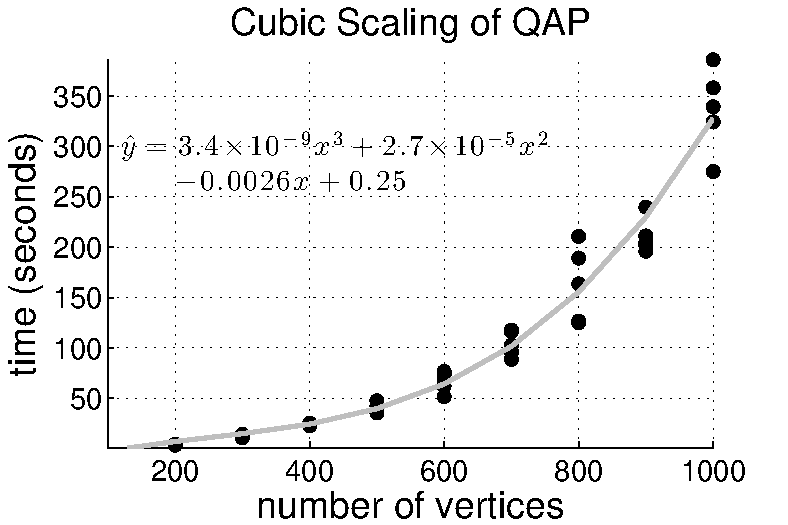
\includegraphics[width=0.5\linewidth]{ErdosRenyi_results.pdf}
	\caption{Running time of \FAQ as function of number of vertices. Data was sampled from an Erd\"os-R\'enyi model with $p=log(n)/n$.  Each dot represents a single simulation, with 100 simulations per $n$.  The solid line is the best fit cubic function.  Note the leading constant is $\dot{\approx} 10^{-9}$ seconds. \FAQ finds the optimal objective function value in every simulation.}
	\label{fig:scaling}
\end{figure}

% subsection algorithm_complexity_and_leading_constants (end)

\subsection{QAP Benchmark Accuracy} % (fold)
\label{sub:qap_benchmarks}

Having demonstrated empirically \texttt{FAQ} has cubic time complexity, we next decided to evaluate its accuracy on a suite of standard benchmarks.  More specifically, QAPLIB is a library of 137 quadratic assignment problems, ranging in size from 10 to 256 vertices \cite{Burkard1997}.  Recent graph matching papers typically evaluate the performance of their algorithm on 16 of the benchmarks that are known to be ``particularly difficult'' \cite{Zaslavskiy2009,Schellewald2001}.  We compare the results of \FAQ to the results of four other state-of-the-art graph matching algorithms: (1) the \texttt{PATH} algorithm, which solves a path between a convex and concave relaxation of QAP \cite{Zaslavskiy2009}, (2) \texttt{QCV} which is the convex relaxation used to initialize the \texttt{PATH} algorithm, (3) the \texttt{RANK} algorithm \cite{Singh2007}, which uses a spectral decomposition, and (4)  the Umeyama algorithm (denoted by \texttt{U} henceforth), which also uses a spectral decomposition \cite{Umeyama1988}.  We chose these four algorithms to compare because the code is freely available from the \texttt{graphm} package \cite{Zaslavskiy2009}.  
% Table \ref{tab:1} shows the results of these 5 algorithms on all 137 benchmarks, along with the optimal values (when they are available).  
Figure \ref{fig:allRelAccuracy} plots the logarithm (base 10, here and elsewhere) of the relative accuracy, that is, $\log_{10}(\mh{f}_{FAQ}/\mh{f}_X)$, for $X \in \{$\texttt{PATH, QCV, RANK, U, all}$\}$, where \texttt{all} is just the best performer of all the non \FAQ algorithms.  Clearly, \FAQ does significantly better than all the other algorithms, outperforming all of them on $\approx 94\%$ of the problems, often by nearly an order of magnitude in terms of relative error.
% Table \ref{tab:1} in the appendix shows the actual objective function values for all the algorithms on each problem.

\begin{figure}[htbp]
	\centering
		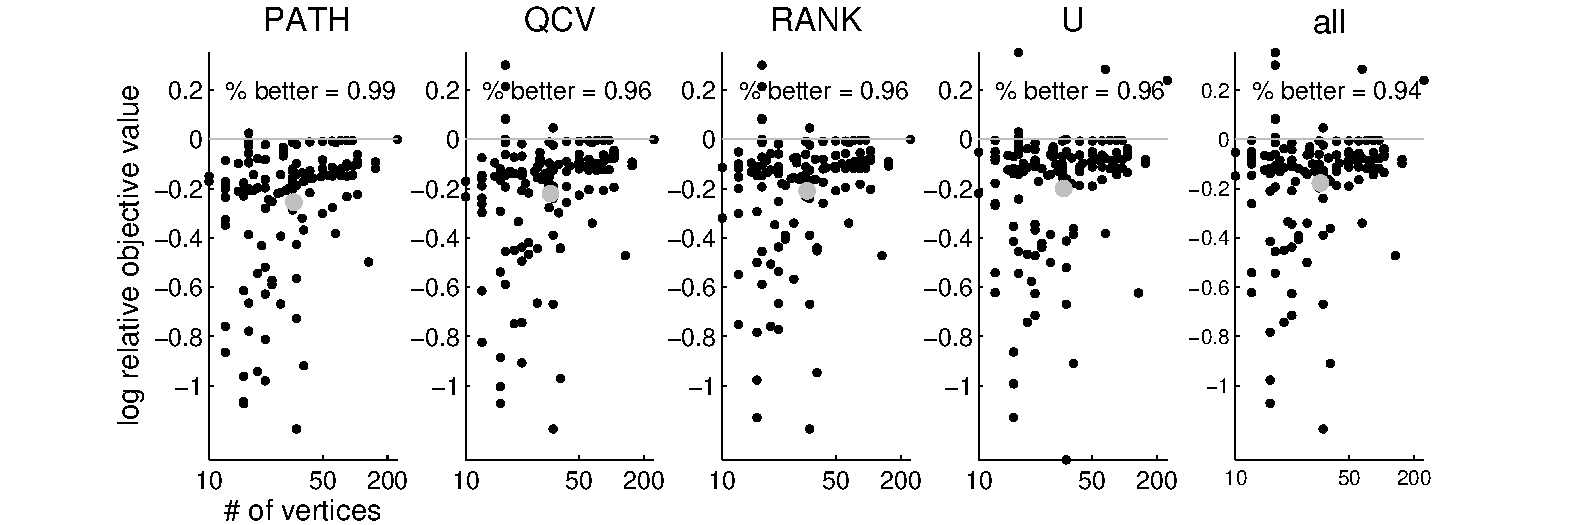
\includegraphics[width=1.0\linewidth]{allRelAccuracy.pdf}
	\caption{Relative accuracy---defined to be $\log_{10}(\mh{f}_{FAQ}/\mh{f}_X)$---of all the four algorithms compared with \texttt{FAQ}.  Note that \FAQ is better than all the other algorithms on $\approx 94\%$ of the benchmarks. The abscissa is the log number of vertices.  The gray dot indicates the mean improvement of \FAQ over the other algorithms.}
	\label{fig:allRelAccuracy}
\end{figure}


% subsection qap_benchmarks (end)

\subsection{QAP Benchmark Efficiency} % (fold)
\label{sub:subsection_name}

As we mentioned in the introduction, the quality of an \emph{approximate} algorithm depends not just on its accuracy, but also its efficiency.  Therefore, we compare the wall time of each of the five algorithms on all 137 benchmarks in Figure \ref{fig:allEfficiency}.  We fit an iteratively weighted least squares linear regression function (Matlab's \texttt{robustfit}) to regress the logarithm of time (in seconds) onto the logarithm of the number of vertices.  The numbers beside the lines indicate the slopes of the regression functions.  The \texttt{PATH} algorithm has the worst slope.  \texttt{QCV} and \FAQ have nearly identical slopes, which makes sense, given that the are solving very similar objective functions.  Similarly, \texttt{RANK} and \texttt{U} have very similar slopes; they are both using spectral approaches.  Note, however, that although the slope of \texttt{RANk} and \texttt{U} are smaller than that of \texttt{FAQ}, they both seem to be super linear on this log-log plot, suggesting that as the number of vertices increases, their compute time might exceed that of the other algorithms.  

\begin{figure}[htbp]
	\centering
		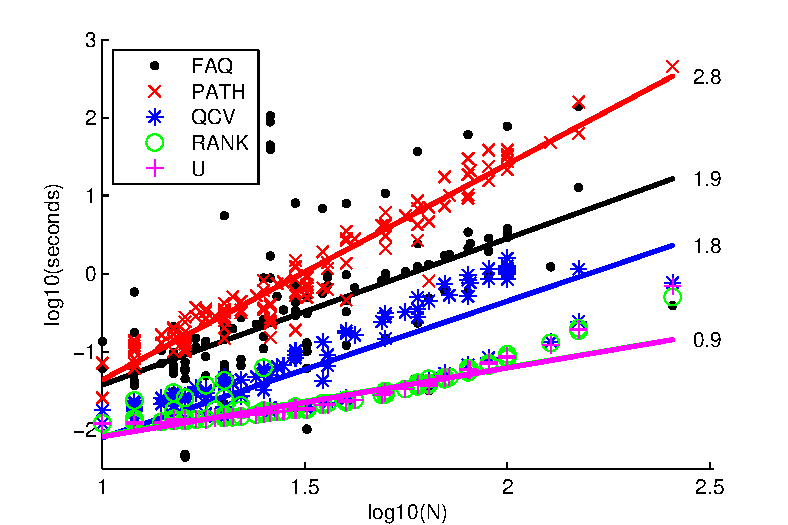
\includegraphics[height=3in]{allEfficiency.pdf}
	\caption{Absolute wall time for running each of the five algorithms on all 137 benchmarks. We fit a line on this log-log plot for each algorithm; the slope is displayed beside each line. The \FAQ slope is much better than the \texttt{PATH} slope, and worse than the others.  Note, however, the time for \texttt{RANK} and \texttt{U} appears to be superlinear on this log-log plot, suggesting that perhaps as the number of vertices increases, \texttt{PATH} might be faster. }
	\label{fig:allEfficiency}
\end{figure}


% subsection subsection_name (end)

\subsection{QAP Benchmark Accuracy/Efficiency Trade-off} % (fold)
\label{sub:qap_benchmark_accuracy_efficiency_trade_off}

In the \texttt{PATH}, the authors demonstrated that \texttt{PATH} outperformed \texttt{QCV} and \texttt{U} on a variety of simulated and real examples in terms of objective function \cite{Zaslavskiy2009}.  If \FAQ yields a lower objective function value than \texttt{FAQ}, and is faster, then it clearly is superior to \texttt{PATH}.  Figure \ref{fig:tradeoff} compares the performance of \FAQ with \texttt{PATH} along both dimensions of performance---accuracy and efficiency---for all 137 benchmarks in the QAPLIB library.  The right panel indicates that \FAQ is both more accurate and more efficient on $80\%$ of the problems.

\begin{figure}[htbp]
	\centering
		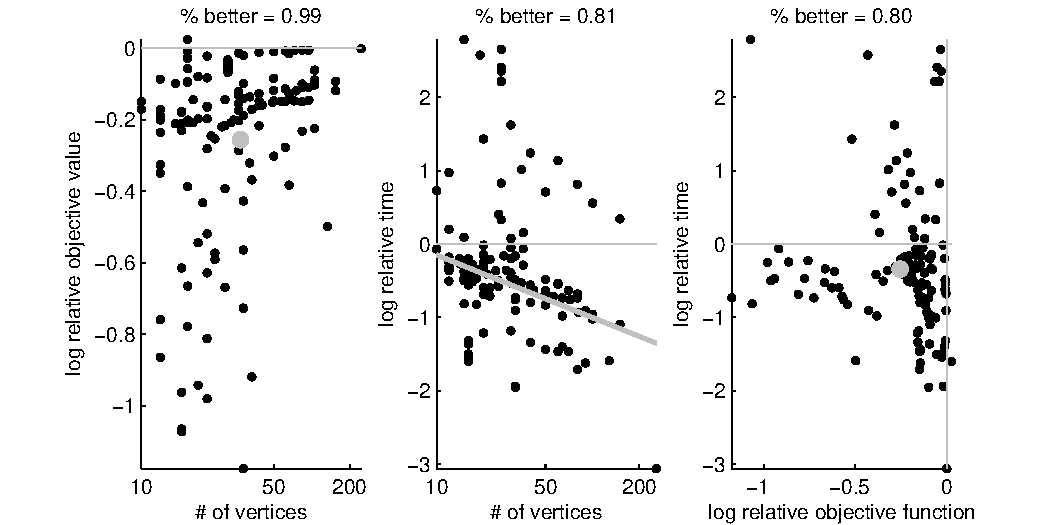
\includegraphics[height=3in]{allPathCompare.pdf}
	\caption{Comparison of \FAQ with \texttt{PATH} in terms of both accuracy and efficiency.  The left panel is the same as the left panel of Figure \ref{fig:allRelAccuracy}.  The middle plots the relative wall time of \FAQ to \texttt{PATH} as a function of the number of vertices, also on a log-log scale.  The gray line is the best fit slope on this plot, suggesting that \FAQ is getting exponentially faster than \texttt{PATH} as the number of vertices gets larger.  Finally, the right panel plots log relative time versus log relative objective function value, demonstrating that \FAQ outperforms \texttt{PATH} on both dimensions on $80\%$ of the benchmarks.}
	\label{fig:tradeoff}
\end{figure}



% subsection qap_benchmark_accuracy_efficiency_trade_off (end)


% 
% \subsection{QAP Undirected Benchmarks}
% \label{sub:undirected}
% 
% We next assess the computational properties of \FAQ in comparison with other the previous state-of-the-art algorithms.  We therefore compare \FAQ to other approaches using a selection of the QAP benchmark library, QAPLIB \cite{Burkard1997}.  Specifically, \cite{Zaslavskiy2009} created a path following algorithm (\texttt{PATH}) based on a convex and concave relaxation of QAP.  In that manuscript, the authors considered 16 datasets from the QAPLIB benchmark, the same 16 datasets as were used in \cite{Schellewald2001}, which are known to be ``particularly difficult''.  \texttt{PATH} was shown to outperform other state-of-the-art algorithms on 14 of 16 tests.  Specifically, \texttt{PATH} was compared to the Quadratic Programming Bound approach (\texttt{QGP}) of \cite{Anstreicher2001}, the graduated assignment algorithm (\texttt{GRAD}) of \cite{Gold1996}, and Umeyama's algorithm (\texttt{U}) \cite{Umeyama1988}.  Because either \texttt{PATH} or \texttt{QBP} outperformed \texttt{GRAD} and \texttt{U} on every dataset, Table \ref{tab:1} shows the performance of \FAQ versus \texttt{PATH} and \texttt{QBP}.  \FAQ outperforms both of the previous state-of-the-art cubic algorithms on 13 out of 16 benchmarks.  Figure \ref{fig:path16} presents the same data graphically. The top panel compares both \FAQ and \texttt{PSOA}---which is the minimum of the previous state-of-the-art (either \texttt{PATH} or \texttt{QBP} here)---to the absolute minimum; \FAQ get closer than \texttt{PSOA} to the minimum on 13 of 16. The bottom panel shows the ratio of \FAQ to \texttt{PSOA}. 
% 
% 
% \begin{table}[h!]
% \caption{Comparison of \FAQ with the optimal objective function value and previous state-of-the-art on a set of 16 standard benchmarks from QAPLIB.  The best (lowest) value is in \textbf{bold}. The number of vertices for each problem is the number in its name (second column).}
% \begin{center}
% \begin{tabular}{|r|r|r||l|l|l|l|l|}
% \hline
% \# & Problem  &   Optimal   & \FAQ & \texttt{PATH} & \texttt{QBP} \\
% \hline
% 1&    chr12c &   11156 &    \textbf{13072} &   18048 	& 20306\\
% 2&    chr15a &    9896 &    27584 &   \textbf{19086} 	& 26132\\
% 3&    chr15c &    9504 &    \textbf{11936}  &   16206 	& 29862\\
% 4&   chr20b &    2298 & \textbf{3068} &    5560 		& 6674\\
% 5&    chr22b &    6194 &    \textbf{8482} &    8500 		& 9942\\
% 6&    esc16b & 292 &    320 & 300 		& \textbf{296}\\
% 7& rou12 &  235528 &    \textbf{253684} &  256320 	& 278834\\
% 8& rou15 &  354210 &    \textbf{371458} &  391270 	& 381016\\
% 9& rou20 &  725522 &    \textbf{743884} &  778284 	& 804676\\
% 10&    tai10a &  135028 &   157954 &  \textbf{152534} 	& 165364\\
% 11&    tai15a &  388214 &   \textbf{397376} &  419224 	& 455778\\
% 12&    tai17a &  491812 &   \textbf{529134} &  530978 	& 550862\\
% 13&    tai20a &  703482 &   \textbf{734276} &  753712 	& 799790\\
% 14&    tai30a & 1818146 &  	\textbf{1894640} & 1903872 	& 1996442\\
% 15&    tai35a & 2422002 & 	\textbf{2460940} & 2555110 	& 2720986\\
% 16&    tai40a & 3139370 &  	\textbf{3227612} & 3281830 	& 3529402\\
% \hline
% \end{tabular}
% \end{center}
% \label{tab:undirected}
% \end{table}%
% 
% 
% \begin{figure}[htbp]
% 	\centering
% 		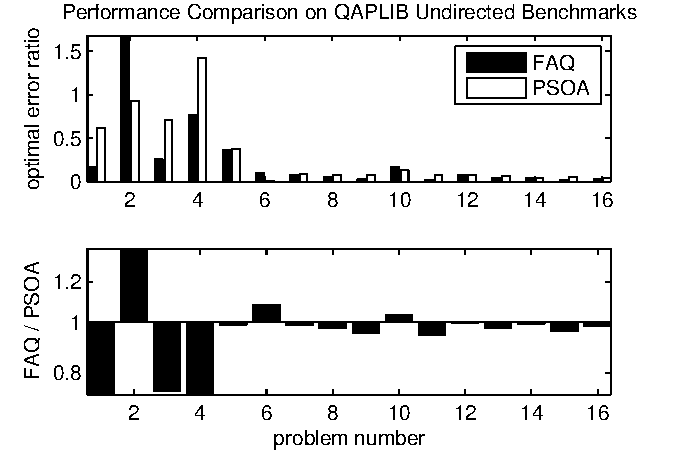
\includegraphics[width=0.5\linewidth]{path16.pdf}
% 	\caption{Performance of \FAQ relative to the previous state-of-the-art (\texttt{PSOA}) algorithms on the undirected QABLIB benchmarks.  Top: The optimal error ratio is defined: $(\mh{f} - f^*)/f^*$, for $\mh{f}$ being the minimum function value found by each algorithm, and $f^*$ is the optimal (minimum) value.  Bottom: Ratio of \FAQ minimum to \texttt{PSOA} minimum.  Note that both panels indicate that \FAQ gets closer to the minimum on 13 of 16 benchmarks.}
% 	\label{fig:path16}
% \end{figure}


\subsection{QAP Directed Benchmarks}
\label{sub:directed}

While this manuscript was under review, Liu et al. \cite{Liu2012} proposed a modification of the \texttt{PATH} algorithm that adjusted \texttt{PATH} to be more appropriate for directed graphs, as the theory motivating the development of \texttt{PATH} relied upon the graphs being undirected.  \texttt{FAQ}, on the other hand, does not depend on the graphs being simple; rather, directed or weighted graphs are both unproblematic. 
% a modification of the \texttt{PATH} algorithm arose that  Nothing in the development of our algorithm depends on the graphs being simple; indeed, \FAQ applies equally well to directed graphs.  To assess the performance of \FAQ on directed graphs, we compare the performance of our algorithm to the previous state-of-the-art. Liu et al.  recently developed an extended path following algorithm for directed graphs \cite{Liu2012}.
Liu et al. compare the performance of their algorithm (\texttt{EPATH}) with \texttt{U}, \texttt{QCV}, and \texttt{GRAD}
on the set of 16 particularly difficult directed benchmarks from QAPLIB.  The \texttt{EPATH} algorithm achieves at least as low objective value as the other algorithms on 15 of 16 benchmarks.  Our algorithm, \texttt{FAQ}, always gets the best of the five algorithms.  Table \ref{tab:directed} shows the numerical results comparing \FAQ to \texttt{EPATH} and \texttt{GRAD}, which sometimes did better than \texttt{EPATH}.  Note that some of the algorithms achieve the absolute minimum on some benchmarks.  
% Figure \ref{fig:lipa16} compares \FAQ to whichever other algorithm did best, clearly indicating that \FAQ is the best on these benchmarks.


\begin{table}[h!]
\caption{Comparison of \FAQ with optimal objective function value and previous state-of-the-art for directed graphs.  The best (lowest) value is in \textbf{bold}. Asterisks indicate achievement of the global minimum.  The number of vertices for each problem is the number in its name (second column).}
\begin{center}
\begin{tabular}{|r|r|r||l|l|l|l|l|}
	\hline 
	          \# &  Problem &      Optimal & \texttt{FAQ} & \texttt{EPATH} & \texttt{GRAD} \\
	\hline 
	           1 &  lipa20a &     3683 & \textbf{3791} &     3885 &     3909 \\ 
	           2 &  lipa20b &    27076 & \textbf{27076}$^*$ &    32081 &    \textbf{27076}$^*$ \\ 
	           3 &  lipa30a &    13178 & \textbf{13571} 	&    13577 &    13668 \\ 
	           4 &  lipa30b &   151426 & \textbf{151426}$^*$ & \textbf{151426}$^*$ &   \textbf{151426}$^*$ \\ 
	           5 &  lipa40a &    31538 & \textbf{32109} 	&    32247 &    32590 \\ 
	           6 &  lipa40b &   476581 & \textbf{476581}$^*$ &   \textbf{476581}$^*$ &   \textbf{476581}$^*$ \\ 
	           7 &  lipa50a &    62093 & \textbf{62962} &    63339 &    63730 \\ 
	           8 &  lipa50b &  1210244 & \textbf{1210244}$^*$ &  \textbf{1210244}$^*$ &  \textbf{1210244}$^*$ \\ 
	           9 &  lipa60a &   107218 & \textbf{108488} &   109168 &   109809 \\ 
	          10 &  lipa60b &  2520135 & \textbf{2520135}$^*$ &  \textbf{2520135}$^*$ &  \textbf{2520135}$^*$ \\ 
	          11 &  lipa70a &   169755 & \textbf{171820} &   172200 &   173172 \\ 
	          12 &  lipa70b &  4603200 & \textbf{4603200}$^*$ &  \textbf{4603200}$^*$ &  \textbf{4603200}$^*$ \\ 
	          13 &  lipa80a &   253195 & \textbf{256073} &   256601 &   258218 \\ 
	          14 &  lipa80b &  7763962 & \textbf{7763962}$^*$ &  \textbf{7763962}$^*$ &  \textbf{7763962}$^*$ \\ 
	          15 &  lipa90a &   360630 & \textbf{363937} &   365233 &   366743 \\ 
	          16 &  lipa90b & 12490441 & \textbf{12490441}$^*$ & \textbf{12490441}$^*$ & \textbf{12490441}$^*$ \\ 
	\hline
	\end{tabular}
\end{center}
\label{tab:directed}
\end{table}%


% \begin{figure}[htbp]
% 	\centering
% 		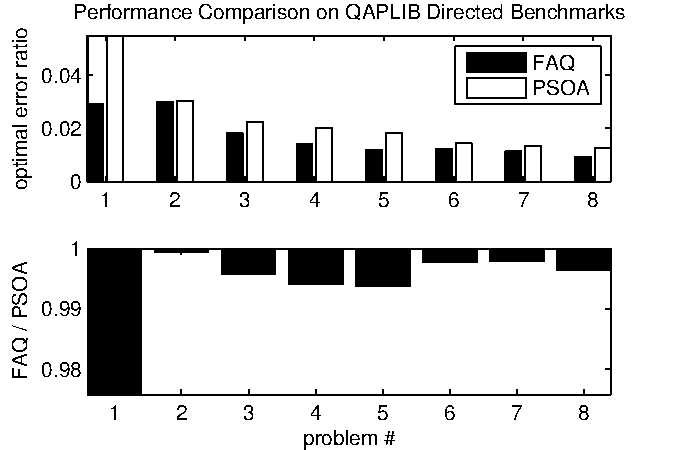
\includegraphics[width=0.5\linewidth]{lipa16.pdf}
% 	\caption{Performance of \FAQ relative to the previous state-of-the-art (\texttt{PSOA}) algorithms on the undirected QABLIB benchmarks. Top and Bottom panels as in Figure \ref{fig:path16}.  Note that \FAQ gets closer to the minimum on all 8 benchmarks for which the \FAQ and \texttt{PSOA} answer differ.}
% 	\label{fig:lipa16}
% \end{figure}
% 


\subsection{Theoretical properties of \FAQ} % (fold)
\label{sub:rqap_solves_qap_}

Although we have no theorems proving error bounds on \texttt{FAQ} relative to the optimal solution, we do have a number of theoretical results to buttress the numerical ones.  As mentioned above in \S \ref{sub:const}, \FAQ is a cubic-time algorithm, as its computational bottleneck is solving the LAPs, which are solved in $\mc{O}(n^3)$ by various algorithms collectively referred to as the ``Hungarian algorithm'' \cite{Jonker1987, Burkard2009}.   

In addition to guarantees on computational time, we have several guarantees on performance.  Consider Eq. \eqref{eq:GM}, and note that Eq. \eqref{eq:trQAP} follows from \eqref{eq:trQAP2} by 
% For example, 
% % Note that rQAP relaxes the constraints of Eq. \eqref{eq:trQAP}, which suggests that 
% in certain important special cases, the minimum of rQAP will be identical to the minimum of QAP. 
% 
%  On the other hand, the equality between Eq. \eqref{eq:trQAP2} and Eq. \eqref{eq:trQAP} follows from 
% 
dropping cross-terms that fall out of the optimization because $P$ is constrained to be a permutation matrix.  \FAQ tries to solve a relaxation of Eq. \eqref{eq:trQAP}, specifically relaxing the permutation matrix constraints to their convex hull.  The resulting objective function, Eq. \eqref{eq:FAQ}, however, is quadratic but not convex.  A different formulation and relaxation of QAP yields a convex objective function. Specifically,
\begin{subequations} \label{eq:rQAP2}
\begin{align} 
		&\underset{P}{\text{minimize}} 		\norm{AP - PB}_F   \label{eq:rQAP2a}\\
		&\text{subject to } 	 P \in \mc{P}, \label{eq:rQAP2b}
\end{align}
\end{subequations}
is also $\mc{NP}$-hard, but upon relaxing \eqref{eq:rQAP2b} to the doubly stochastic matrices, the result is convex \cite{Almohamad1993}.  Thus, a linear programming algorithm is guaranteed to find the optimal solution to Eq. \eqref{eq:rQAP2}.  This relaxation is in fact the objective function that \texttt{QCV} is solving.  

If we had relaxed the constraints prior to canceling those terms, this equality would not follow.  This leads us to wonder in which circumstances are the objective functions of QAP and rQAP equal.  The following lemma clarifies:
 % This insight leads to the following theorem:
% Although, rLAP and LAP are always equivalent, in general, it is not the case that FAQ and QAP are equivalent.  However, in a certain important special case, FAQ and QAP are equivalent.
\begin{lem}
	If $A$ and $B$ are the adjacency matrices of simple graphs (symmetric, hollow, and binary) that are isomorphic to one another, then the minimum of rQAP is equal to the minimum of QAP.
\end{lem}
\begin{proof}
Because any feasible solution to QAP is also a feasible solution to rQAP, we must only show that the optimal objective function value to rQAP can be no better than the optimal objective function value of QAP.  Let $A=PBP\T$, so that $\langle A, PBP\T\rangle=2m$, where $m$ is the number of edges in $A$.  If rQAP could achieve a lower objective value, then it must be that there exists a $D \in \mc{D}$ such that $\langle A, DBD\T\rangle > \langle A, PBP\T\rangle = 2m$ (remember that we are minimizing the negative Euclidean inner product). For that to be the case, it must be that $(DBD\T)_{ij} \geq 1$ for some $(u,v)$.  That this is not so may be seen by the submultiplicativity of the norm induced by the $\ell_{\infty}$ norm:
$\norm{Dx}_\infty \leq \norm{D}_{\infty,\infty} \norm{x}_\infty$.  Applying this twice (once for each doubly stochastic matrix multiplication) yields our result.
% Consider $d_i=\langle D, \text{col}_i(BD\T) \rangle$, where $\text{col}_i(\cdot)$ indicates the $i^{th}$ column of the matrix.  $d_i \leq 1$ for all $i \in [n]$, therefore, our result holds.
\end{proof}
% subsection rqap_solves_qap_ (end)


% section theoretical_results (end)

% \section{Numerical Results} % (fold)
% \label{sub:numerical_results}


% subsection numerical_results (end)


\subsection{Multiple Restarts} % (fold)
\label{sub:multiple_restarts}

Although \FAQ outperformed all other algorithms on nearly every benchmark, that \FAQ was not always the best was annoying to us.
% . \texttt{PSOA} on 13 of 16 undirected benchmarks, and always did the best amongst 16 of 16 directed benchmarks, it was annoying to us that we did not do best on all 32 benchmarks.  
% Note that the computational bottleneck of both \FAQ and \texttt{PATH} is the Hungarian algorithm which solves a LAP. 
% \FAQ strives to solve a non-convex problem.
% In \texttt{PATH}, the algorithm finds the minimum of a convex path between two extremes, $F_0$ and $F_1$.  Similarly, \texttt{QBP} finds the minimum of a convex program.  Our approach, on the other hand, does not construct a convex problem to solve, rather, it chooses an initial starting point and then finds a local optimum (note that the initial position of the \texttt{PATH} algorithm could also be variable, because $F_0$ is not convex as they assert, so their starting point depends on their initialization). 
% 
We therefore utilized the non-convexity of rQAP is as a feature, although it can equally well be regarded as a bug  (because rQAP is non-convex so the solution found by \FAQ depends on the initial condition).  We can utilize the non-convexity as a feature, however, whenever (i) we have some reason to believe that better solutions exist (many algorithms efficiently compute relatively tight lower bounds \cite{Anstreicher2009}), and (ii) we can efficiently search the space of initial conditions.  Although we lack any supporting theory of optimality, we do know how to sample feasible starting points.  Specifically, we desire that our starting points are ``near'' the flat matrix, and satisfy the conditions.  Therefore, we  sample $K \in \mc{D}$, a random doubly stochastic matrix using 10 iterations of Sinkhorn balancing \cite{Sinkhorn1964}, and let our initial guess be $P^{(0)}=(J+K)/2$, where $J$ is the doubly flat matrix.  We can therefore use any number of restarts with this approach.  Fixing the number of restarts, we still have a cubic time algorithm, although the constants change.  

Table \ref{tab:restarts} shows the performance of running \FAQ 3 and 100 times, reporting only the best result (indicated by \texttt{FAQ}$_3$ and \texttt{FAQ}$_{100}$, respectively), and comparing it to the best performing result of the five algorithms (running only \FAQ once). Note that we only consider the 16 particularly difficult benchmarks for this evaluation. \FAQ only required three restarts to outperform all other approximate algorithms on all 16 of 16 difficult benchmarks.  Moreover, after 100 restarts, \FAQ finds the absolute minimum on 3 of the 16 benchmarks; none of the other algorithms ever achieved the absolute minimum on any of these benchmarks. 
% Figure \ref{fig:restarts} graphically demonstrates these results. 
 % Note that restarting \FAQ a fixed number of multiple times is still cubic.  Future work could investigate performance as a function of the number of restarts. %, although with an arbitrary number of random restarts, stating that it is cubic is somewhat meaningless.  



\begin{table}[h!]
\caption{Comparison of \FAQ with optimal objective function value and the best result  on the undirected benchmarks.  Note that \FAQ restarted 100 times finds the optimal objective function value in 3 of 16 benchmarks, and that \FAQ restarted 3 times finds a minimum better than the previous state-of-the-art on all 16 particularly difficult benchmarks.}
\begin{center}
\begin{tabular}{|r|r|r||l|l|l|l|l|}
\hline
\# & Problem  &   Optimal    & \texttt{FAQ}$_{100}$ & \texttt{FAQ}$_{3}$ & previous min \\
\hline
1&    chr12c &   11156 &    \textbf{12176} &   13072 & 13072 \\
2&    chr15a &    9896 &    \textbf{9896}$^*$ &   17272 &  19086 \\
3&    chr15c &    9504 &    \textbf{10960} &   14274 &  16206 \\
4&   chr20b &    2298 &     \textbf{2786} &    3068 &    3068 \\
5&    chr22b &    6194 &    \textbf{7218} &    7876 &   8482 \\
6&    esc16b & 	292 & 		\textbf{292}$^*$ & 294 &    296 \\
7& 	   rou12 &  235528 &  \textbf{235528}$^*$ &  238134 &    253684 \\
8& 	   rou15 &  354210 &  \textbf{356654} &  371458 &    371458 \\
9&      rou20 &  725522 &  \textbf{730614} &  743884 &    743884 \\
10&    tai10a &  135028 &  \textbf{135828} &  148970 &    152534 \\
11&    tai15a &  388214 &  \textbf{391522} &  397376 &    397376 \\
12&    tai17a &  491812 &  \textbf{496598} &  511574 &    529134 \\
13&    tai20a &  703482 &  \textbf{711840} &  721540 &    734276 \\
14&    tai30a & 1818146 & \textbf{1844636} & 1890738 &  1894640 \\
15&    tai35a & 2422002 & \textbf{2454292} & 2460940 &  2460940 \\
16&    tai40a & 3139370 & \textbf{3187738} & 3194826 &  3227612 \\
    \hline
\end{tabular}
\end{center}
\label{tab:restarts}
\end{table}%

% \begin{figure}[htbp]
% 	\centering
% 		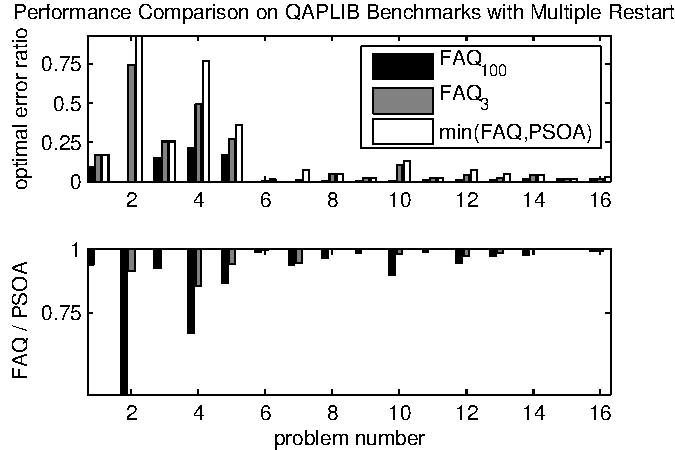
\includegraphics[width=0.5\linewidth]{path16_restarts.pdf}
% 	\caption{Performance of \FAQ with multiple restarts on the undirected benchmarks. \texttt{FAQ}$_3$ yields a lower objective function value than the best result from Figure \ref{fig:path16}, and \texttt{FAQ}$_{100}$ finds the absolute optimal permutation on 3 of the 16 benchmarks.  Note that no other algorithm compared ever found the optimal for any of the benchmarks.}
% 	\label{fig:restarts}
% \end{figure}


% subsection multiple_restarts (end)

% 
% \begin{figure}[htbp]
% 	\centering			
% 	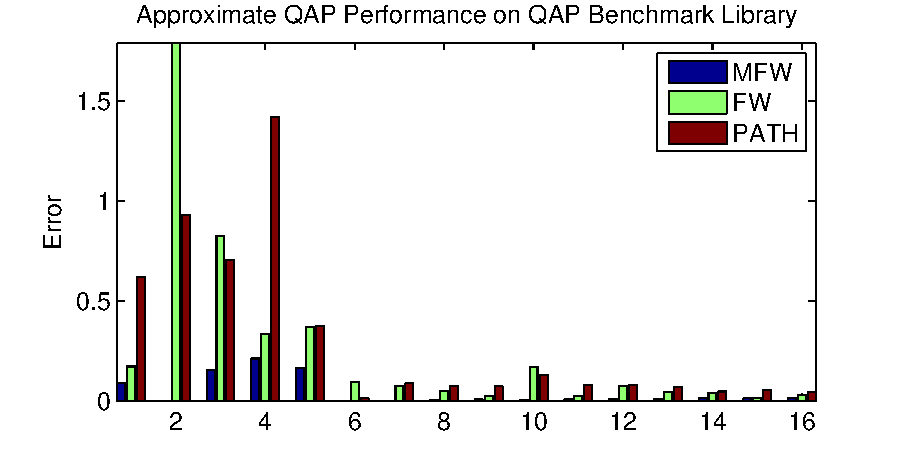
\includegraphics[width=1.0\linewidth]{benchmarks.pdf}
% 	\caption{\texttt{FAQ}$_3$ outperforms the previous state-of-the-art (PSOA) on all 16 benchmark graph matching problems.  Moreover, \FAQa outperforms PSOA on 12 of 16 tests.  For 3 of 16 tests, \FAQb achieves the minimum (none of the other algorithms ever find the absolute minimum), as indicated by a black dot.  Let $f_*$ be the minimum and $\mh{f}_x$ be the minimum achieved by algorithm $x$.  Error is $\mh{f}_x/f_*-1$.  }
% 	\label{fig:fwpath}
% \end{figure}



\subsection{Brain-Graph Matching} % (fold)
\label{sub:connectome_classification}

A ``chemical connectome'' is a brain-graph in which vertices correspond to (collections of) neurons, and edges correspond to chemical synapses between them. The \emph{Caenorhabditis elegans} (\emph{C. elegans}) is a small worm (nematode) with $302$ labeled vertices.  We consider the subgraph with $279$ somatic neurons that form edges with other neurons \cite{WhiteBrenner86, Varshney2011}.  
% Though vertices in brain-graphs can connect via either chemical or electrical synapses, the chemical connectome is the connectome of primary interest

% Two distinct kinds of edges exist between vertices: chemical and electrical ``synapses'' (edges). Any pair of vertices may have several edges of each type. Moreover, some of the synapses are hyper-edges amongst more than two vertices.  
Because pairs of neurons sometimes have multiple synapses between them, and they are directed, the chemical connectome of \emph{C. elegans} may be thought of as a weighted directed graph.
 % Thus, the connectome of a \emph{C. elegans} may be thought of as a weighted multi-hypergraph, where the weights are the number of edges of each type.  \FAQ natively operates on weighted or unweighted graphs.  
We therefore conducted the following synthetic experiments.  
Let $A_{ij} \in \{0,1,2,\ldots\}$ be the number of synapses from neuron $i$ to neuron $j$, and let $A=\{A_{ij}\}_{i,j \in [279]}$.  To generate synthetic data, we let $B^{(k)}=Q^{(k)} A {Q^{(k)}}\T$, for some $Q^{(k)}$ chosen uniformly at random from $\mc{P}$, effectively shuffling the vertex labels of the connectome.  Then, we try to graph match $A$ to $B^{(k)}$, for  $k =1,2,\ldots, 1000$, that is, we repeat the experiment $1000$ times.  We define accuracy as the fraction of vertices correctly assigned. We always start with the doubly flat matrix.


\begin{figure}[htbp]
	\centering
		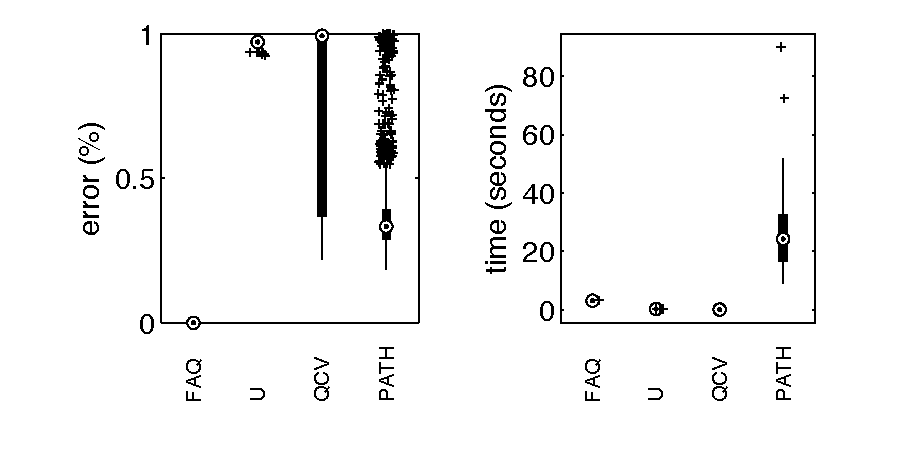
\includegraphics[width=0.5\linewidth]{chemicalConnectome.pdf}
	\caption{Performance of \texttt{U}, \texttt{QCV}, \texttt{PATH}, and \FAQ on synthetic C.~elegans connectome data, that is, graph matching the true connectomes with permuted versions of themselves.  Error is the fraction of vertices correctly matched.  Circle indicates the median, thick black bars indicate the quartiles, thin black lines indicate extreme but non-outlier points, and plus signs are outliers. The left panel indicate error (fraction of misassigned vertices), and the right panel indicates wall time on a 2.2 GHz Apple MacBook.   \FAQ always obtained the optimal solution, whereas none of the other algorithms ever found the optimal.    \FAQ also ran very quickly, nearly as quickly as \texttt{U} and \texttt{QCV}, and much faster than \texttt{PATH}, even though the \FAQ implementation is in Matlab, and the others are in C.}
	\label{fig:connectomes}
\end{figure}


Figure \ref{fig:connectomes} displays the results of \FAQ along with \texttt{U}, \texttt{QCV},  and \texttt{PATH}.  The left panel indicates that \FAQ \emph{always} found the optimal solution for the chemical connectome, whereas none of the other algorithms \emph{ever} found the optimal solution.  The right panel compares the wall time of the various algorithms, running on an 2.2 GHz Apple MacBook. Note that we have only a Matlab implementation of \texttt{FAQ}, whereas the other algorithms are implemented in C.  Nonetheless, \FAQ runs nearly as quickly as both \texttt{U} and \texttt{QCV}, and significantly faster than \texttt{PATH}.  %This suggests that lower level language implementation of \FAQ might be 

% The properties of this connectomes are analyzed in \cite{Varshney2011}; a cursory evaluation of the properties of these graphs does not suggest to us why the chemical connectome was so much easier to graph match than the electrical one. 


To investigate the performance of \FAQ on undirected graphs, we ran \FAQ on binarized symmeterized versions of the graphs ($A_{ij}=1$ if and only if $A_{ij}\geq 1$ or $A_{ji} \geq 1$).  The resulting errors are nearly identical to those presented in Figure \ref{fig:connectomes}, although speed increased by greater than a factor of two. Note that the number of vertices in this brain-graph matching problem---279---is larger than the largest of the 137 benchmarks used above. 




\section{Discussion}
\label{sec:discussion}

This work presents a fast approximate quadratic assignment problem algorithm called \FAQ for approximately solving large graph matching problems, motivated by brain-graphs.  Our key insight was to relax the binary constraint of QAP to its continuous and non-negative counterpart---the doubly stochastic matrix---which is the convex hull of the original feasible region.  
Numerically, we demonstrated that not only is \FAQ cubic in time, but also its leading constants are quite small---$10^{-9}$---suggesting that it can be used for graphs with hundreds or thousands of vertices.  
Moreover, it achieves better accuracy than previous state-of-the-art approximate algorithms on on over $93\%$ of the 137 QAPLIB benchmarks, including both directed and undirected graph matching problems.  Because rQAP is non-convex, we also consider multiple restarts, and achieve improved performance for the particularly difficult benchmarks using only two or three restarts.  We then demonstrate that the solution to our relaxed optimization problem, rQAP, is identical to that for QAP whenever the two graphs are simple and isomorphic to one another.  Finally, we used it to match C.~elegans connectomes to permuted versions of themselves. Of the four state-of-the-art algorithms considered, \FAQ achieved perfect performance $100\%$ of the time, whereas none of the other three algorithms ever achieved perfect performance.  Moreover, \FAQ ran about as fast as two of them, and significantly faster than \texttt{PATH}, even though \FAQ is implemented in Matlab, and the others are implemented in C.  Note that these connectomes have 279 vertices, more vertices than even the largest benchmarks. 


Fortunately, our work is not done. Even with very small leading constants for this algorithm, as $n$ increases, the computational burden gets quite high.  For example, extrapolating the curve of Figure \ref{fig:scaling}, this algorithm would take about 20 years to finish (on a standard laptop from 2011) when $n=100,000$.  We hope to be able to approximately solve rQAP on graphs much larger than that, given that the number of neurons even in a fly brain, for example, is $\approx 250,000$.  More efficient algorithms and/or implementations are required for such massive graph matching. Although a few other state-of-the-art algorithms were more efficient than \texttt{FAQ}, their accuracy was significantly worse.  So the search continues to find approximate graph matching algorithms with scaling rules like \texttt{QCV}, \texttt{U} or \texttt{RANK}, but performance like \texttt{FAQ}.


Additional future work might generalize \FAQ in a number of ways.  First, many (brain-) graphs of interest will be errorfully observed \cite{Priebe2011}, that is, vertices might be missing and putative edges might exhibit both false positives and negatives.  Explicitly dealing with this error source is both theoretically and practically of interest \cite{VP11_unlabeled}.  
Second, for many brain-graph matching problems, the number of vertices will not be the same across the brains.  Recent work from \cite{Zaslavskiy2009, Zaslavskiy2010} and \cite{Escolano2011} suggest that extensions in this direction would be both relatively straightforward and effective. Third, the most ``costly'' subroutine is LAP.  Fortunately, LAP is a quadratic optimization problem with linear constraints.  A number of parallelized optimization strategies could therefore potentially be brought to bear on this problem \cite{Boyd2011}.  Fourth, our matrices have certain special properties, namely sparsity, which makes more efficient algorithms (such as ``active set'' algorithms) readily available for further speed increases.  Fifth, for brain-graphs, we have some prior information that could easily be incorporated in the form of vertex attributes.  For example, position in the brain, cell type, etc., could be used to measure ``dissimilarity'' between vertices.  %The WGMP could easily incorporate these dissimilarities, in fact, the original QAP formulation already encodes them via the matrix $C$; that matrix was simply dropped when WGMP was originally proposed.  
% The objective function could then be modified to give
% \begin{align} \label{eq:Jqap}
% 	\mt{Q}_{AB}= \argmin_{Q \in \mc{D}} \norm{Q A Q\T - B}^2_F + \lambda J(Q),
% \end{align}
% where $J(Q)$ is a dissimilarity based penalty and $\lambda$ is a hyper-parameter.  
Finally, although this approach natively operates on both unweighted and weighted graphs, multi-graphs are a possible extension.

In conclusion, this manuscript has presented an algorithm for approximately solving the quadratic assignment problem that is fast, effective, and easily generalizable.  Yet, the $\mc{O}(n^3)$ complexity remains too slow to solve many problems of interest.  To facilitate further development and applications, all the code and data used in this manuscript is available from the first author's website, \url{http://jovo.me}.

% \subsection{Related Problems} % (fold)
% \label{sub:related_problems}
% 
% In addition to brain-graph matching, large approximate graph matching could be fruitful for a number of other domains.  For example, consider social networks.  In both the Twitter and Facebook graph, each vertex represents an individual.  For many users of each social networking application, it is not clear whether they have an account on another social network, and if so, what is the label of that account.  Thus, graph matching in this domain could suggest assignments of Facebook user names to twitter accounts.  Alternately, consider a language graph, where each vertex represent a word in some language, and an edge represent the existence of an adjacency between a pair of words in a text corpus of that language.  If one could match a pair of graphs corresponding to two different languages, one might obtain a highly effective machine translation tool. This might be especially true when no additional information is known about one or both languages.
% 
% Consider the scale of these problems.  Twitter and Facebook have $\mc{O}(10^8)$ users and languages often have $\mc{O}(10^5)$ words.  Exact graph matching algorithms require exponential time in the worst case.  So, even considering the smallest problem above, brain-graph matching, the fastest exact graph matching algorithms would require more time than there are nanoseconds since the big bang.\footnote{Assuming the big bang occurred 15 billion years ago means about $10^{17}$ seconds ago.  Assuming computational time is $1.004^n$ nanoseconds, even when $n=10^4$, the problem will already exceed the number of seconds since the big bang} This motivates us to consider developing \emph{approximate} (or \emph{heuristic}) algorithms, with polynomial time complexity.  Indeed, we present here an algorithm the requires approximately one week on a standard desktop computer (running non-optimized code) to match graphs with $\mc{O}(10^4)$ vertices.
% 
% 
% % subsection related_problems (end)


\appendix
\newpage
% \textbf{APPENDIX}

% \section{QAPLIB Benchmark Results} % (fold)
% \label{sec:qaplib_benchmark_results}
% 
% 
% 
% \begin{table}[h!]
% \caption{Comparison of \FAQ with the optimal objective function value and previous state-of-the-art on the entire set of 137 benchmarks from QAPLIB.  The best (lowest) value is in \textbf{bold}. The number of vertices for each problem is the number in its name (second column).  When the optimal objective function is unknown, we write ``NaN''.}
% \begin{center}
% \begin{tabular}{|r|r|r||l|l|l|l|l|l|}
% \hline
% \# & Problem  &   Optimal   & \FAQ & \texttt{PATH} & \texttt{QCV} & \texttt{RANK} & \texttt{U} \\
% \hline
% 1 & bur26a & 5.43e+06 & \textbf{5.43e+06} & 5.85e+06 & 6.56e+06 & 6.67e+06 & 6.41e+06 \\ 
% 2 & bur26b & 3.82e+06 & \textbf{3.83e+06} & 4.24e+06 & 4.7e+06 & 4.74e+06 & 4.15e+06 \\ 
% 3 & bur26c & 5.43e+06 & \textbf{5.44e+06} & 6.27e+06 & 6.17e+06 & 6.58e+06 & 5.86e+06 \\ 
% 4 & bur26d & 3.82e+06 & \textbf{3.83e+06} & 4.2e+06 & 4.61e+06 & 4.68e+06 & 4.19e+06 \\ 
% 5 & bur26e & 5.39e+06 & \textbf{5.4e+06} & 5.86e+06 & 6.67e+06 & 6.71e+06 & 6.11e+06 \\ 
% 6 & bur26f & 3.78e+06 & \textbf{3.78e+06} & 4.42e+06 & 4.77e+06 & 4.71e+06 & 4.35e+06 \\ 
% 7 & bur26g & 1.01e+07 & \textbf{1.01e+07} & 1.12e+07 & 1.21e+07 & 1.21e+07 & 1.14e+07 \\ 
% 8 & bur26h & 7.1e+06 & \textbf{7.12e+06} & 8.06e+06 & 8.68e+06 & 8.73e+06 & 7.64e+06 \\ 
% 9 & chr12a & 9.55e+03 & \textbf{3.3e+04} & 7.38e+04 & 5.72e+04 & 5.23e+04 & 3.34e+04 \\ 
% 10 & chr12b & 9.74e+03 & \textbf{1.05e+04} & 7.66e+04 & 6.98e+04 & 5.9e+04 & 4.38e+04 \\ 
% 11 & chr12c & 1.12e+04 & \textbf{1.31e+04} & 7.5e+04 & 5.4e+04 & 4.61e+04 & 4.55e+04 \\ 
% 12 & chr15a & 9.9e+03 & \textbf{2.65e+04} & 1.09e+05 & 9.17e+04 & 8.38e+04 & 6.88e+04 \\ 
% 13 & chr15b & 7.99e+03 & \textbf{9.11e+03} & 1.06e+05 & 9.21e+04 & 8.64e+04 & 8.97e+04 \\ 
% 14 & chr15c & 9.5e+03 & \textbf{1.19e+04} & 1.1e+05 & 9.18e+04 & 7.25e+04 & 8.72e+04 \\ 
% 15 & chr18a & 1.11e+04 & \textbf{1.54e+04} & 1.35e+05 & 8.66e+04 & 8.87e+04 & 8.54e+04 \\ 
% 16 & chr18b & 1.53e+03 & \textbf{1.66e+03} & 5.79e+03 & 4.67e+03 & 5.31e+03 & 4.85e+03 \\ 
% 17 & chr20a & 2.19e+03 & \textbf{2.53e+03} & 1.64e+04 & 1.4e+04 & 1.17e+04 & 1.07e+04 \\ 
% 18 & chr20b & 2.3e+03 & \textbf{4.06e+03} & 1.72e+04 & 1.11e+04 & 1.11e+04 & 1.2e+04 \\ 
% 19 & chr20c & 1.41e+04 & \textbf{1.98e+04} & 1.9e+05 & 1.6e+05 & 1.18e+05 & 1.03e+05 \\ 
% 20 & chr22a & 6.16e+03 & \textbf{8.29e+03} & 3.23e+04 & 2.42e+04 & 2.03e+04 & 2.19e+04 \\ 
% 21 & chr22b & 6.19e+03 & \textbf{8.42e+03} & 3.15e+04 & 2.21e+04 & 2.14e+04 & 2.31e+04 \\ 
% 22 & chr25a & 3.8e+03 & \textbf{6.28e+03} & 2.93e+04 & 2.9e+04 & 2.32e+04 & 1.99e+04 \\ 
% 23 & els19 & 1.72e+07 & \textbf{2.13e+07} & 5.76e+07 & 4.6e+07 & 4.74e+07 & 8.03e+07 \\ 
% 24 & esc128 & 64 & \textbf{68} & 214 & 202 & 202 & 286 \\ 
% 26 & esc16b & 292 & 320 & 326 & 320 & 320 & \textbf{314} \\ 
% 28 & esc16d & 16 & \textbf{16} & 74 & 62 & 62 & 56 \\ 
% 29 & esc16e & 28 & \textbf{32} & 78 & 50 & 50 & 56 \\ 
% 30 & esc16f & 0 & \textbf{0} & 0 & 0 & 0 & 0 \\ 
% 33 & esc16i & 14 & \textbf{14} & 84 & 40 & 40 & 40 \\ 
% 34 & esc16j & 8 & 36 & 34 & 22 & 22 & \textbf{16} \\ 
% 35 & esc32a & NaN & \textbf{150} & 550 & 368 & 368 & 498 \\ 
% 36 & esc32b & NaN & \textbf{184} & 492 & 320 & 320 & 476 \\ 
% 38 & esc32d & NaN & \textbf{322} & 404 & 340 & 340 & 362 \\ 
% 39 & esc32e & 2 & \textbf{2} & 30 & 30 & 30 & 40 \\ 
% 40 & esc32f & 2 & \textbf{2} & 30 & 30 & 30 & 40 \\ 
% 41 & esc32g & 6 & \textbf{6} & 32 & 28 & 28 & 28 \\ 
% 42 & esc32h & NaN & \textbf{472} & 726 & 630 & 630 & 686 \\ 
% \hline
% \end{tabular}
% \end{center}
% \label{tab:1}
% \end{table}%
% 
% \begin{table}[h!]
% % \caption{Comparison of \FAQ with the optimal objective function value and previous state-of-the-art on the entire set of 137 benchmarks from QAPLIB.  The best (lowest) value is in \textbf{bold}. The number of vertices for each problem is the number in its name (second column).}
% \begin{center}
% \begin{tabular}{|r|r|r||l|l|l|l|l|l|}
% \hline
% \# & Problem  &   Optimal   & \FAQ & \texttt{PATH} & \texttt{QCV} & \texttt{RANK} & \texttt{U} \\
% \hline
% 43 & esc64a & NaN & \textbf{116} & 280 & 254 & 254 & 280 \\ 
% 44 & had12 & 1.65e+03 & \textbf{1.68e+03} & 2.05e+03 & 2e+03 & 1.9e+03 & 1.89e+03 \\ 
% 45 & had14 & 2.72e+03 & \textbf{2.72e+03} & 3.42e+03 & 3.39e+03 & 3.4e+03 & 3.17e+03 \\ 
% 46 & had16 & 3.72e+03 & \textbf{3.73e+03} & 4.62e+03 & 4.3e+03 & 4.41e+03 & 4.29e+03 \\ 
% 47 & had18 & 5.36e+03 & \textbf{5.43e+03} & 6.51e+03 & 6.42e+03 & 6.21e+03 & 5.94e+03 \\ 
% 48 & had20 & 6.92e+03 & \textbf{6.98e+03} & 8.45e+03 & 8.17e+03 & 8.01e+03 & 7.7e+03 \\ 
% 49 & kra30a & 8.89e+04 & \textbf{9.47e+04} & 1.25e+05 & 1.43e+05 & 1.47e+05 & 1.33e+05 \\ 
% 50 & kra30b & 9.14e+04 & \textbf{9.7e+04} & 1.31e+05 & 1.51e+05 & 1.46e+05 & 1.38e+05 \\ 
% 51 & kra32 & 8.89e+04 & \textbf{9.57e+04} & 1.33e+05 & 1.48e+05 & 1.41e+05 & 1.39e+05 \\ 
% 52 & lipa20a & 3.68e+03 & \textbf{3.79e+03} & 3.98e+03 & 3.96e+03 & 3.96e+03 & 3.93e+03 \\ 
% 53 & lipa20b & 2.71e+04 & \textbf{2.71e+04} & 3.93e+04 & 3.8e+04 & 3.68e+04 & 3.5e+04 \\ 
% 54 & lipa30a & 1.32e+04 & \textbf{1.36e+04} & 1.4e+04 & 1.39e+04 & 1.38e+04 & 1.38e+04 \\ 
% 55 & lipa30b & 1.51e+05 & \textbf{1.51e+05} & 2.16e+05 & 2.05e+05 & 1.96e+05 & 1.98e+05 \\ 
% 56 & lipa40a & 3.15e+04 & \textbf{3.21e+04} & 3.29e+04 & 3.28e+04 & 3.28e+04 & 3.27e+04 \\ 
% 57 & lipa40b & 4.77e+05 & \textbf{4.77e+05} & 6.87e+05 & 6.45e+05 & 6.29e+05 & 6.18e+05 \\ 
% 58 & lipa50a & 6.21e+04 & \textbf{6.3e+04} & 6.44e+04 & 6.41e+04 & 6.4e+04 & 6.4e+04 \\ 
% 59 & lipa50b & 1.21e+06 & \textbf{1.21e+06} & 1.7e+06 & 1.6e+06 & 1.59e+06 & 1.57e+06 \\ 
% 60 & lipa60a & 1.07e+05 & \textbf{1.08e+05} & 1.1e+05 & 1.1e+05 & 1.1e+05 & 1.1e+05 \\ 
% 61 & lipa60b & 2.52e+06 & \textbf{2.52e+06} & 3.55e+06 & 3.36e+06 & 3.3e+06 & 3.27e+06 \\ 
% 62 & lipa70a & 1.7e+05 & \textbf{1.72e+05} & 1.74e+05 & 1.74e+05 & 1.74e+05 & 1.74e+05 \\ 
% 63 & lipa70b & 4.6e+06 & \textbf{4.6e+06} & 6.45e+06 & 6.16e+06 & 6.05e+06 & 6.06e+06 \\ 
% 64 & lipa80a & 2.53e+05 & \textbf{2.56e+05} & 2.59e+05 & 2.59e+05 & 2.59e+05 & 2.58e+05 \\ 
% 65 & lipa80b & 7.76e+06 & \textbf{7.76e+06} & 1.1e+07 & 1.03e+07 & 1.02e+07 & 1.02e+07 \\ 
% 66 & lipa90a & 3.61e+05 & \textbf{3.64e+05} & 3.68e+05 & 3.67e+05 & 3.67e+05 & 3.68e+05 \\ 
% 67 & lipa90b & 1.25e+07 & \textbf{1.25e+07} & 1.75e+07 & 1.66e+07 & 1.64e+07 & 1.64e+07 \\ 
% 68 & nug12 & 578 & \textbf{598} & 1.03e+03 & 838 & 850 & 902 \\ 
% 69 & nug14 & 1.01e+03 & \textbf{1.07e+03} & 1.74e+03 & 1.51e+03 & 1.45e+03 & 1.43e+03 \\ 
% 70 & nug15 & 1.15e+03 & \textbf{1.18e+03} & 2.01e+03 & 1.73e+03 & 1.66e+03 & 1.63e+03 \\ 
% 71 & nug16a & 1.61e+03 & \textbf{1.65e+03} & 2.66e+03 & 2.27e+03 & 2.11e+03 & 2.29e+03 \\ 
% 72 & nug16b & 1.24e+03 & \textbf{1.32e+03} & 2.1e+03 & 1.86e+03 & 1.86e+03 & 1.75e+03 \\ 
% 73 & nug17 & 1.73e+03 & \textbf{1.76e+03} & 2.84e+03 & 2.43e+03 & 2.41e+03 & 2.38e+03 \\ 
% 74 & nug18 & 1.93e+03 & \textbf{1.99e+03} & 3.13e+03 & 2.74e+03 & 2.65e+03 & 2.6e+03 \\ 
% 75 & nug20 & 2.57e+03 & \textbf{2.63e+03} & 4.14e+03 & 3.65e+03 & 3.63e+03 & 3.2e+03 \\ 
% 76 & nug21 & 2.44e+03 & \textbf{2.44e+03} & 4.29e+03 & 3.69e+03 & 3.69e+03 & 3.62e+03 \\ 
% 77 & nug22 & 3.6e+03 & \textbf{3.63e+03} & 6.51e+03 & 6e+03 & 5.59e+03 & 4.77e+03 \\ 
% 78 & nug24 & 3.49e+03 & \textbf{3.55e+03} & 5.89e+03 & 4.79e+03 & 5.13e+03 & 4.97e+03 \\ 
% 79 & nug25 & 3.74e+03 & \textbf{3.75e+03} & 6.17e+03 & 5.37e+03 & 5.37e+03 & 5.21e+03 \\ 
% 80 & nug27 & 5.23e+03 & \textbf{5.35e+03} & 8.64e+03 & 7.8e+03 & 7.78e+03 & 6.75e+03 \\ 
% 81 & nug28 & 5.17e+03 & \textbf{5.22e+03} & 8.28e+03 & 7.2e+03 & 7.4e+03 & 7.02e+03 \\ 
% 82 & nug30 & 6.12e+03 & \textbf{6.18e+03} & 9.85e+03 & 8.83e+03 & 8.59e+03 & 7.79e+03 \\ 
% 83 & rou12 & 2.36e+05 & \textbf{2.53e+05} & 3.76e+05 & 3.68e+05 & 3.33e+05 & 2.98e+05 \\ 
% 84 & rou15 & 3.54e+05 & \textbf{3.71e+05} & 5.61e+05 & 5.33e+05 & 4.89e+05 & 4.87e+05 \\ 
% 85 & rou20 & 7.26e+05 & \textbf{7.44e+05} & 1.09e+06 & 1.04e+06 & 9.62e+05 & 9.34e+05 \\ 
% 86 & scr12 & 3.14e+04 & \textbf{3.36e+04} & 7.09e+04 & 6.65e+04 & 6.72e+04 & 6.12e+04 \\ 
% 87 & scr15 & 5.11e+04 & \textbf{6.21e+04} & 1.01e+05 & 1.22e+05 & 1.22e+05 & 1.4e+05 \\ 
% 88 & scr20 & 1.1e+05 & \textbf{1.17e+05} & 2.24e+05 & 1.9e+05 & 2.09e+05 & 2.74e+05 \\ 
% \hline
% \end{tabular}
% \end{center}
% \label{tab:2}
% \end{table}%
% 
% 
% \begin{table}[h!]
% % \caption{Comparison of \FAQ with the optimal objective function value and previous state-of-the-art on the entire set of 137 benchmarks from QAPLIB.  The best (lowest) value is in \textbf{bold}. The number of vertices for each problem is the number in its name (second column).}
% \begin{center}
% \begin{tabular}{|r|r|r||l|l|l|l|l|l|}
% \hline
% \# & Problem  &   Optimal   & \FAQ & \texttt{PATH} & \texttt{QCV} & \texttt{RANK} & \texttt{U} \\
% \hline
% 89 & sko100a & 1.52e+05 & \textbf{1.54e+05} & 1.92e+05 & 1.82e+05 & 1.87e+05 & 1.79e+05 \\ 
% 90 & sko100b & 1.54e+05 & \textbf{1.56e+05} & 1.97e+05 & 1.86e+05 & 1.88e+05 & 1.8e+05 \\ 
% 91 & sko100c & 1.48e+05 & \textbf{1.49e+05} & 1.88e+05 & 1.78e+05 & 1.82e+05 & 1.74e+05 \\ 
% 92 & sko100d & 1.5e+05 & \textbf{1.52e+05} & 1.91e+05 & 1.78e+05 & 1.81e+05 & 1.75e+05 \\ 
% 93 & sko100e & 1.49e+05 & \textbf{1.51e+05} & 1.9e+05 & 1.8e+05 & 1.83e+05 & 1.78e+05 \\ 
% 94 & sko100f & 1.49e+05 & \textbf{1.51e+05} & 1.9e+05 & 1.78e+05 & 1.79e+05 & 1.75e+05 \\ 
% 95 & sko42 & NaN & \textbf{1.62e+04} & 2.33e+04 & 2.08e+04 & 2.12e+04 & 2.02e+04 \\ 
% 96 & sko49 & NaN & \textbf{2.37e+04} & 3.36e+04 & 3e+04 & 3.05e+04 & 2.92e+04 \\ 
% 97 & sko56 & NaN & \textbf{3.46e+04} & 4.87e+04 & 4.47e+04 & 4.36e+04 & 4.2e+04 \\ 
% 98 & sko64 & NaN & \textbf{4.9e+04} & 6.57e+04 & 6.11e+04 & 6.18e+04 & 5.86e+04 \\ 
% 99 & sko72 & NaN & \textbf{6.69e+04} & 8.8e+04 & 8.37e+04 & 8.22e+04 & 8.14e+04 \\ 
% 100 & sko81 & 9.1e+04 & \textbf{9.19e+04} & 1.18e+05 & 1.13e+05 & 1.12e+05 & 1.1e+05 \\ 
% 101 & sko90 & 1.16e+05 & \textbf{1.16e+05} & 1.49e+05 & 1.39e+05 & 1.42e+05 & 1.4e+05 \\ 
% 102 & ste36a & 9.53e+03 & \textbf{1.05e+04} & 2.44e+04 & 2.91e+04 & 2.89e+04 & 2.41e+04 \\ 
% 103 & ste36b & 1.59e+04 & \textbf{1.71e+04} & 1.42e+05 & 1.6e+05 & 1.52e+05 & 1.39e+05 \\ 
% 104 & ste36c & 8.24e+06 & \textbf{8.79e+06} & 1.3e+07 & 2.43e+07 & 2.49e+07 & 2.14e+07 \\ 
% 105 & tai100a & 2.11e+07 & \textbf{2.17e+07} & 2.66e+07 & 2.48e+07 & 2.41e+07 & 2.42e+07 \\ 
% 106 & tai100b & 1.19e+09 & \textbf{1.25e+09} & 2.09e+09 & 1.96e+09 & 1.99e+09 & 1.71e+09 \\ 
% 107 & tai10a & NaN & \textbf{1.58e+05} & 2.34e+05 & 2.34e+05 & 2.06e+05 & 1.78e+05 \\ 
% 108 & tai10b & NaN & \textbf{1.39e+06} & 1.96e+06 & 2.38e+06 & 2.9e+06 & 2.3e+06 \\ 
% 109 & tai12a & 2.24e+05 & \textbf{2.45e+05} & 3.78e+05 & 3.78e+05 & 3.19e+05 & 2.98e+05 \\ 
% 110 & tai12b & 3.95e+07 & \textbf{4.99e+07} & 7.92e+07 & 9.13e+07 & 6.29e+07 & 9.25e+07 \\ 
% 111 & tai150b & 4.99e+08 & \textbf{5.14e+08} & 6.76e+08 & 6.59e+08 & 6.59e+08 & 6.43e+08 \\ 
% 112 & tai15a & 3.88e+05 & \textbf{3.97e+05} & 5.97e+05 & 5.24e+05 & 5.12e+05 & 4.68e+05 \\ 
% 113 & tai15b & 5.18e+07 & \textbf{5.2e+07} & 6.15e+08 & 6.15e+08 & 7.02e+08 & 7.02e+08 \\ 
% 114 & tai17a & 4.92e+05 & \textbf{5.29e+05} & 7.38e+05 & 7.13e+05 & 6.44e+05 & 6.62e+05 \\ 
% 115 & tai20a & 7.03e+05 & \textbf{7.36e+05} & 1.07e+06 & 9.95e+05 & 9.76e+05 & 8.96e+05 \\ 
% 116 & tai20b & 1.22e+08 & \textbf{1.39e+08} & 4.6e+08 & 4.35e+08 & 4.8e+08 & 3.08e+08 \\ 
% 118 & tai25a & 1.17e+06 & \textbf{1.22e+06} & 1.7e+06 & 1.59e+06 & 1.46e+06 & 1.41e+06 \\ 
% 119 & tai25b & 3.44e+08 & \textbf{3.69e+08} & 9.11e+08 & 1.02e+09 & 8.06e+08 & 8.96e+08 \\ 
% 120 & tai30a & NaN & \textbf{1.89e+06} & 2.51e+06 & 2.37e+06 & 2.18e+06 & 2.22e+06 \\ 
% 121 & tai30b & 6.37e+08 & \textbf{7.15e+08} & 1.38e+09 & 1.35e+09 & 1.22e+09 & 1.13e+09 \\ 
% 122 & tai35a & NaN & \textbf{2.46e+06} & 3.36e+06 & 3.11e+06 & 2.97e+06 & 2.93e+06 \\ 
% 123 & tai35b & 2.83e+08 & \textbf{3.06e+08} & 6.39e+08 & 6.08e+08 & 4.44e+08 & 4.62e+08 \\ 
% 124 & tai40a & NaN & \textbf{3.23e+06} & 4.32e+06 & 3.97e+06 & 3.89e+06 & 3.74e+06 \\ 
% 125 & tai40b & 6.37e+08 & \textbf{6.68e+08} & 1.1e+09 & 1.2e+09 & 1.22e+09 & 1.03e+09 \\ 
% 126 & tai50a & 4.94e+06 & \textbf{5.13e+06} & 6.73e+06 & 6.22e+06 & 5.96e+06 & 5.9e+06 \\ 
% 127 & tai50b & 4.59e+08 & \textbf{4.77e+08} & 9.54e+08 & 8.03e+08 & 7.71e+08 & 7.39e+08 \\ 
% 128 & tai60a & 7.21e+06 & \textbf{7.44e+06} & 9.67e+06 & 8.97e+06 & 8.48e+06 & 8.63e+06 \\ 
% 129 & tai60b & 6.08e+08 & \textbf{6.47e+08} & 1.23e+09 & 1.04e+09 & 1.02e+09 & 9.45e+08 \\ 
% 130 & tai64c & 1.86e+06 & 5.7e+06 & 5.89e+06 & 5.89e+06 & 5.89e+06 & \textbf{2.96e+06} \\ 
% \hline
% \end{tabular}
% \end{center}
% \label{tab:3}
% \end{table}%
% 
% \begin{table}[h!]
% % \caption{Comparison of \FAQ with the optimal objective function value and previous state-of-the-art on the entire set of 137 benchmarks from QAPLIB.  The best (lowest) value is in \textbf{bold}. The number of vertices for each problem is the number in its name (second column).}
% \begin{center}
% \begin{tabular}{|r|r|r||l|l|l|l|l|l|}
% \hline
% \# & Problem  &   Optimal   & \FAQ & \texttt{PATH} & \texttt{QCV} & \texttt{RANK} & \texttt{U} \\
% \hline
% 131 & tai80a & 1.35e+07 & \textbf{1.39e+07} & 1.74e+07 & 1.61e+07 & 1.57e+07 & 1.57e+07 \\ 
% 132 & tai80b & 8.18e+08 & \textbf{8.5e+08} & 1.45e+09 & 1.37e+09 & 1.29e+09 & 1.19e+09 \\ 
% 133 & tho150 & 8.13e+06 & \textbf{8.22e+06} & 1.02e+07 & 1.02e+07 & 1.01e+07 & 9.93e+06 \\ 
% 134 & tho30 & 1.5e+05 & \textbf{1.53e+05} & 2.28e+05 & 2.31e+05 & 2.25e+05 & 2.09e+05 \\ 
% 135 & tho40 & 2.41e+05 & \textbf{2.5e+05} & 3.5e+05 & 3.89e+05 & 3.73e+05 & 3.38e+05 \\ 
% 136 & wil100 & 2.73e+05 & \textbf{2.75e+05} & 3.16e+05 & 3.05e+05 & 3.07e+05 & 3e+05 \\ 
% 137 & wil50 & NaN & \textbf{4.93e+04} & 5.98e+04 & 5.66e+04 & 5.74e+04 & 5.55e+04 \\ 
% \hline
% \end{tabular}
% \end{center}
% \label{tab:4}
% \end{table}%
% 
% % section qaplib_benchmark_results (end)

\clearpage
\section{Linear Assignment Problems} % (fold)
% \label{ssub:linear_assignment_problems}

% subsubsection linear_assignment_problems (end)

The standard way of writing a Linear Assignment Problem (LAP) is
\begin{subequations} \label{eq:LAP}
\begin{align}
	 \text{(LAP) }\quad  &\underset{\pi}{\text{minimize}} \sum_{u,v \in [n]} a_{u \pi(v)} b_{ij} \\
	&\text{subject to } \pi \in \Pi,
\end{align}
\end{subequations}
which can be written equivalently in a number of ways using the notion of permutation matrix introduced in the main text:
\begin{subequations} \label{eq:LAP2}
\begin{align}
	&\argmin_{\PmcP} \norm{PA - B}_F =\\
	&\argmin_{\PmcP} \, tr(PA-B)\T (PA-B)=\\ 
	% &\argmin_{\PmcP} tr (A\T P\T PA) - tr(2PAB\T) + tr(B\T B)=\\ 
	&\argmin_{\PmcP}  -tr (P AB\T) = \argmin_{\PmcP}  -\langle P\T, AB\T \rangle = \label{eq:2c} \\
	% &\argmin_{\PmcP}  -\sum_{u,v \in [n]} p_{ij} a_{ij} b_{ji}
	% =\\% &\argmin_{\PmcP}  - \text{vec}(P)\T \text{vec}(AB\T).=\\
	&\argmin_{\PmcP}  -\langle P, AB\T \rangle, \label{eq:dotLAP}
\end{align}
\end{subequations}
where $\langle \cdot,\cdot \rangle$ %the equality on the second to last line defines 
is the usual Euclidean inner product, i.e., $\langle X,Y\rangle \defn tr(X\T Y)= \sum_{ij} x_{ij} y_{ij}$.
While the objective function and the first two constraints of LAP are linear, the binary constraints make solving even this problem computationally tricky.  Nonetheless, in the last several decades, there has been much progress in accelerating algorithms for solving LAPs, starting with exponential time, all the way down to $\mc{O}(n^3)$ for general LAPs, and even faster for certain special cases (e.g., sparse matrices) \cite{Jonker1987, Burkard2009}.

That Eq. \eqref{eq:dotFW1} is a LAP is evident by considering Eq. \eqref{eq:dotLAP}.  If $A=\nabla_P^{(i)}$ and $B=I$ (the $n\times n$ identity matrix), then Eq. \eqref{eq:dotFW1} is identical to Eq. \eqref{eq:dotLAP}.


% The last form indicates that LAP is a linear programming problem (hence the name).  Yet, the constraints, $\mc{P}$, make it a bit trickier.  The feasible region $\mc{P}$ can be written as a set of three constraints: two linear equality constraint sets and a binary constraint.  The LAP objection function with constraints can explicitly be written:
% \begin{align}
% 		&\text{minimize}_P  &&\sum_{u \in \mc{V}} -p_{ij} a_{ij} b_{ji} \nonumber \\
% 		&\text{subject to } && \sum_{u \in \mc{V}} p_{ij} = 1 \, \forall u \in \mc{V} \nonumber \\
% 		& && \sum_{v \in \mc{V}} p_{ij} = 1 \, \forall v \in \mc{V}, \nonumber \\
% 		& &&p_{ij} \in \{0,1\} \, \forall u,v. \label{eq:rLAP}	
% \end{align}
% Perhaps because LAP comes up in a wide variety of contexts, a large number of algorithms have been developed to solve LAP \cite{Burkard2009}.  These algorithms have become increasing efficient.  
% One of the most popular algorithms, the so-called ``Hungarian algorithm'' has time complexity $\mc{O}(n^3)$ \cite{Jonker1987}.  Under certain conditions (for example, when $AB\T$ is sparse), faster implementations are also available.  As will be seen below, LAP is a key subroutine to our inexact QAP solution.  

To solve a LAP, consider a continuous relaxation of LAP, specifically, relaxing the permutation matrix constraint to a doubly stochastic matrix constraint:
% A matrix $P$ is doubly stochastic precisely when $P$ satisfies the following three conditions: 
% \begin{enumerate}
% \item	$P\mb{1} = \mb{1}$,
% \item	$P\T \mb{1}=\mb{1}$, %\\
% \item 	$P \in  \Real_+^{n \times n}$,
% \end{enumerate}
% where the third constraint relaxes the binary constraints of the permutation matrices with a non-negativity constraint.  
% Let $\mc{D}$ be the set of doubly stochastic matrices.
% With this, we now state a relaxed LAP problem:
\begin{subequations} \label{eq:rLAP}
\begin{align}
		\text{(rLAP) } \quad &\underset{P}{\text{minimize}}  &&-\langle P, AB\T \rangle \\
		&\text{subject to } && P \in \mc{D}.
		% && \sum_{u \in \mc{V}} p_{ij} = 1 \, \forall u \in \mc{V} \nonumber \\
		% 		& && \sum_{v \in \mc{V}} p_{ij} = 1 \, \forall v \in \mc{V}, \nonumber \\
		% 		& &&p_{ij} \geq 0 \, \forall u,v, \label{eq:ALAP}	
\end{align}
\end{subequations}
As it turns out, solving rLAP is equivalent to solving LAP.
\begin{prop}
	LAP and rLAP are equivalent, meaning that they have the same optimal objective function value.
\end{prop}
\begin{proof}
	Although this proposition is typically proven by invoking total unimodularity, we present a simpler proof here.	Let $P'$ be a solution to LAP and let $P = \sum_{i\in[k]} \alpha_i P^{(i)}$ be a solution to rLAP for some positive integer $k$, permutation matrices $\{P^{(i)}\}_{i \in [k]}$, and positive real numbers $\{\alpha_i\}_{i \in[k]}$ such that $\sum_{i \in [k]} \alpha_i=1$.  Note that 
	\begin{align*}
	\langle P,AB\T \rangle &= \langle  \sum_{i\in[k]} \alpha_i P^{(i)}, AB\T \rangle=  \sum_{i\in[k]} \alpha_i \langle  P^{(i)}, AB\T \rangle	 \\
	&\leq \sum_{i\in[k]} \alpha_i \langle P', AB\T  \rangle = \langle P', AB\T \rangle \leq \langle P, AB\T \rangle,
	\end{align*}
	% then we have a contradiction, 
	because $P'$ is feasible in rLAP.
	\end{proof}
This relaxation motivates our approach to approximating QAP.

	



\section*{Acknowledgment}

The authors would like to acknowledge two helpful reviewers as well as Lav Varshney for providing the data. This work was partially supported by the Research Program in Applied Neuroscience. 


\bibliographystyle{unsrt}


\begin{thebibliography}{10}

\bibitem{Conte2004}
D~Conte, P~Foggia, C~Sansone, and M~Vento.
\newblock {THIRTY YEARS OF GRAPH MATCHING IN PATTERN RECOGNITION}.
\newblock {\em International Journal of Pattern Recognition and Artificial
  Intelligence}, 18(3):265--298, 2004.

\bibitem{Papadimitriou1998}
Christos~H Papadimitriou and Kenneth Steiglitz.
\newblock {\em {Combinatorial Optimization: Algorithms and Complexity}}.
\newblock Dover Publications, 1998.

\bibitem{Burkard1997}
Rainer~E Burkard, Stefan~E Karisch, and Franz Rendl.
\newblock {QAPLIB – A Quadratic Assignment Problem Library}.
\newblock {\em Journal of Global Optimization}, 10(4):391--403, 1997.

\bibitem{SpornsKotter05}
Olaf Sporns, Giulio Tononi, and R~Kotter.
\newblock {The Human Connectome: A Structural Description of the Human Brain}.
\newblock {\em PLoS Computational Biology}, 1(4):e42, 2005.

\bibitem{Hagmann05}
Patric Hagmann.
\newblock {\em {From diffusion MRI to brain connectomics}}.
\newblock PhD thesis, Institut de traitement des signaux, 2005.

\bibitem{Zuo2011}
Xi-nian~N Zuo, Ross Ehmke, Maarten Mennes, Davide Imperati, Francisco~Xavier
  Castellanos, Olaf Sporns, and Michael~Peter Milham.
\newblock {Network Centrality in the Human Functional Connectome.}
\newblock {\em Cerebral cortex (New York, N.Y. : 1991)}, pages bhr269--,
  October 2011.

\bibitem{Csernansky2004}
John~G Csernansky, Lei Wang, Sarang~C Joshi, J~Tilak Ratnanather, and Michael~I
  Miller.
\newblock {Computational anatomy and neuropsychiatric disease: probabilistic
  assessment of variation and statistical inference of group difference,
  hemispheric asymmetry, and time-dependent change.}
\newblock {\em NeuroImage}, 23 Suppl 1:S56--68, January 2004.

\bibitem{Kubicki2007}
Marek Kubicki, Robert McCarley, Carl-Fredrik Westin, Hae-Jeong Park, Stephan
  Maier, Ron Kikinis, Ferenc~A Jolesz, and Martha~E Shenton.
\newblock {A review of diffusion tensor imaging studies in schizophrenia.}
\newblock {\em Journal of Psychiatric Research}, 41(1-2):15--30, 2007.

\bibitem{Calhoun2011}
Vince~D. Calhoun, Jing Sui, Kent Kiehl, Jessica~A Turner, Elena~a Allen, and
  Godfrey Pearlson.
\newblock {Exploring the psychosis functional connectome: aberrant intrinsic
  networks in schizophrenia and bipolar disorder.}
\newblock {\em Frontiers in psychiatry / Frontiers Research Foundation}, 2:75,
  January 2011.

\bibitem{Fornito2012}
Alex Fornito and Edward~T. Bullmore.
\newblock {Connectomic intermediate phenotypes for psychiatric disorders.}
\newblock {\em Frontiers in psychiatry / Frontiers Research Foundation}, 3:32,
  January 2012.

\bibitem{Fornito2012a}
Alex Fornito, Andrew Zalesky, Christos Pantelis, and Edward~T. Bullmore.
\newblock {Schizophrenia, neuroimaging and connectomics}.
\newblock {\em NeuroImage}, February 2012.

\bibitem{VP11_unlabeled}
Joshua~T Vogelstein and Carey~E Priebe.
\newblock {Shuffled Graph Classification: Theory and Connectome Applications}.
\newblock {\em Submitted to IEEE PAMI}, 2011.

\bibitem{Duin2011}
Robert P~W Duin, Elżbieta Pękalska, and Elżbieta Pękalskab.
\newblock {The dissimilarity space: Bridging structural and statistical pattern
  recognition}.
\newblock {\em Pattern Recognition Letters}, in press(April), May 2011.

\bibitem{Fortin1996}
Scott Fortin.
\newblock {The Graph Isomorphism Problem}.
\newblock {\em Technical Report, University of Alberta, Dept of CS}, 1996.

\bibitem{Babai1980}
L\'{a}szl\'{o} Babali, Paul Erdős, and Stanley~M Selkow.
\newblock {RANDOM GRAPH ISOMORPHISM}.
\newblock {\em SIAM Journal on Computing}, 9(August):628--635, 1980.

\bibitem{Babai1981}
L\'{a}szl\'{o} Babali.
\newblock {Moderately Exponential Bound for Graph Isomorphism}.
\newblock {\em Fundamentals of Computation Theory}, pages 34--50, August 1981.

\bibitem{Chen1994}
Jianer Chen.
\newblock {A Linear-Time Algorithm for Isomorphism of Graphs of Bounded Average
  Genus}.
\newblock {\em SIAM Journal on Discrete Mathematics}, 7(4):614, November 1994.

\bibitem{Frank1956}
M~Frank and P~Wolfe.
\newblock {An Algorithm for Quadratic Programming}.
\newblock {\em Naval Research Logistics Quarterly}, 3(1-2):95--110, 1956.

\bibitem{Bradley1977}
Stephen~P Bradley, Arnoldo~C Hax, and Thomas~L Magnanti.
\newblock {\em {Applied Mathematical Programming}}.
\newblock Addison-Wesley, 1977.

\bibitem{Anstreicher03}
Kurt~M. Anstreicher.
\newblock {Recent advances in the solution of quadratic assignment}.
\newblock {\em SIAM Journal on Optimization}, 97(1-2):27--42, 2003.

\bibitem{Burkard2009}
Rainer~E Burkard, Mauro Dell'Amico, and Silvano Martello.
\newblock {\em {Assignment Problems}}.
\newblock SIAM, 2009.

\bibitem{Kuhn1955}
H.~W. Kuhn.
\newblock {The Hungarian method for the assignment problem}.
\newblock {\em Naval Research Logistics Quarterly}, 2(1-2):83--97, March 1955.

\bibitem{Konig1931}
D\'{e}nes Kőnig.
\newblock {Gr\'{a}fok \'{e}s M\'{a}trixok}.
\newblock {\em Matematikai \'{e}s Fizikai Lapok}, 38:116--119, 1931.

\bibitem{Egevary1931}
Jenő Egev\'{a}ry.
\newblock {Matrixok kombinatorius tulajdons\'{a}gair\'{o}l}.
\newblock {\em Matematikai \'{e}s Fizikai Lapok}, 38:16--28, 1931.

\bibitem{Jonker1987}
R~Jonker and A~Volgenant.
\newblock {A shortest augmenting path algorithm for dense and sparse linear
  assignment problems}.
\newblock {\em Computing}, 38(4):325--340, 1987.

\bibitem{Zaslavskiy2009}
Mikhail Zaslavskiy, Francis~R Bach, and Jean-philippe~P Vert.
\newblock {A path following algorithm for the graph matching problem}.
\newblock {\em IEEE Transactions on Pattern Analysis and Machine Intelligence},
  31(12):2227--2242, 2009.

\bibitem{Schellewald2001}
Christian Schellewald, Stefan Roth, and Christoph Schn\"{o}rr.
\newblock {Evaluation of Convex Optimization Techniques for the Weighted
  Graph-Matching Problem in Computer Vision}.
\newblock In {\em Proceedings of the 23rd DAGMSymposium on Pattern
  Recognition}, pages 361--368. Springer-Verlag, 2001.

\bibitem{Singh2007}
Rohit Singh, Jinbo Xu, and Bonnie Berger.
\newblock {Pairwise global alignment of protein interaction networks by
  matching neighborhood topology}.
\newblock {\em RESEARCH IN COMPUTATIONAL MOLECULAR BIOLOGY}, 4453:16--31, April
  2007.

\bibitem{Umeyama1988}
Shinji Umeyama.
\newblock {An Eigendecomposition Approach to Weighted Graph Matching Problems}.
\newblock {\em Analysis}, I(5), 1988.

\bibitem{Liu2012}
Zhi-Yong Liu, Hong Qiao, and Lei Xu.
\newblock {An Extended Path Following Algorithm for Graph Matching Problem.}
\newblock {\em IEEE transactions on pattern analysis and machine intelligence},
  34(7):1451--1456, January 2012.

\bibitem{Almohamad1993}
H~A Almohamad and S~O Duffuaa.
\newblock {A linear programming approach for the weighted graph matching
  problem}.
\newblock {\em IEEE Transactions on Pattern Analysis and Machine Intelligence},
  15(5):522--525, 1993.

\bibitem{Anstreicher2009}
Kurt~M. Anstreicher.
\newblock {Semidefinite programming versus the reformulation-linearization
  technique for nonconvex quadratically constrained quadratic programming}.
\newblock {\em Journal of Global Optimization}, pages 471--484, 2009.

\bibitem{Sinkhorn1964}
R~Sinkhorn.
\newblock {A relationship between arbitrary positive matrices and doubly
  stochastic matrices}.
\newblock {\em The Annals of Mathematical Statistics}, 35(2):876--879, 1964.

\bibitem{WhiteBrenner86}
J~White, E~Southgate, J.~Nichol Thomson, and S~Brenner.
\newblock {The structure of the nervous system of the nematode caenorhabditis
  elegans.}
\newblock {\em Philosophical Transactions of Royal Society London. Series B,
  Biological Sciences}, 314(1165):1--340, 1986.

\bibitem{Varshney2011}
Lav~R Varshney, Beth~L Chen, Eric Paniagua, David~H Hall, Dmitri~B. Chklovskii,
  Cold Spring, and Janelia Farm.
\newblock {Structural Properties of the Caenorhabditis elegans Neuronal
  Network}.
\newblock {\em PLoS Computational Biology}, 7(2):1--41, February 2011.

\bibitem{Priebe2011}
Carey~E Priebe, Joshua~T Vogelstein, and Davi~D Bock.
\newblock {Optimizing the quantity/quality trade-off in connectome inference}.
\newblock {\em Communications in Statistics Theory and Methods}, page~7, 2011.

\bibitem{Zaslavskiy2010}
Mikhail Zaslavskiy, Francis~R Bach, and Jean-philippe~P Vert.
\newblock {Many-to-Many Graph Matching: A Continuous Relaxation Approach}.
\newblock {\em Machine Learning and Knowledge Discovery in Databases},
  6323:515--530, 2010.

\bibitem{Escolano2011}
Francisco Escolano, Edwin Hancock, and Miguel Lozano.
\newblock {Graph Matching through Entropic Manifold Alignment}.
\newblock {\em Computer Vision and Pattern Recognition}, 2011.

\bibitem{Boyd2011}
Stephen Boyd, Neal Parikh, Eric Chu, Borja Peleato, and Jonathan Eckstein.
\newblock {Foundations and Trends in Machine Learning}.
\newblock {\em Foundations and Trends in Machine Learning}, 3(1):1--122, 2011.

\end{thebibliography}




\end{document}



